\documentclass[journal]{IEEEtran}
\usepackage{amsmath,amsfonts}
% \usepackage{algorithmic}
\usepackage{algorithm}
\usepackage[noend]{algpseudocode}
\usepackage{array}
\usepackage[caption=false,font=scriptsize,labelfont=sf,textfont=sf]{subfig}
\usepackage{textcomp}
\usepackage{stfloats}
\usepackage{hyperref}
\usepackage{url}
\usepackage{verbatim}
\usepackage{graphicx}
\usepackage{marginnote}
\usepackage{multicol}
\usepackage{multirow}
\usepackage{makecell}
\usepackage[acronym,sort=standard,nonumberlist]{glossaries}

\renewcommand{\arraystretch}{1.5}

%\usepackage{dblfloatfix} % To enable figures at the bottom of page

\hyphenation{op-tical net-works semi-conduc-tor IEEE-Xplore}
\def\BibTeX{{\rm B\kern-.05em{\sc i\kern-.025em b}\kern-.08em
    T\kern-.1667em\lower.7ex\hbox{E}\kern-.125emX}}
\usepackage{balance}
\usepackage[table,xcdraw,svgnames,dvipsnames]{xcolor}

\usepackage{tikz-related}

\providecommand{\atB  }[1]{\textcolor{red}{@Basem:~}\textcolor{blue}{#1}}

\makeatletter
% Reinsert missing \algbackskip
\def\algbackskip{\hskip-\ALG@thistlm}
\makeatother

\begin{document}
\title{Generating Synthetic Vehicle Data Using Decentralized Generative Adversarial Networks}
\author{Basem Shaker$^{1}$, Gastone Pietro Rosati Papini$^{1,*}$, Matteo Saveriano$^{1}$, and Kuo-Yun Liang$^{2}$
\thanks{$^{1}$Department of Industrial Engineering, University of Trento, Trento, Italy.}
\thanks{$^{*}$Corresponding author: {\footnotesize{\tt gastone.rosatipapini@unitn.it}}.}
\thanks{$^{2}$Scania CV AB, Södertälje, Sweden.}}

%\markboth{Journal of \LaTeX\ Class Files,~Vol.~18, No.~9, September~2020}%
%{How to Use the IEEEtran \LaTeX \ Templates}

\maketitle

\newacronym{gan}{GAN}{Generative Adversarial Network}

\newacronym{ann}{ANN}{Artificial Neural Network}

\newacronym{cnn}{CNN}{Convolutional Neural Network}

\newacronym{aps}{APS}{Air Processing System}

\newacronym{bce}{BCE}{Binary Cross Entropy}

\newacronym{mse}{MSE}{Mean Square Error}

\newacronym{iid}{IID}{Independent and Identically Distributed}

\newacronym{niid}{non-IID}{non-Independent and Identically Distributed}

\newacronym{ml}{ML}{Machine Learning}

\newacronym{lstm}{LSTM}{Long Short Term Memory}

\newacronym{is}{IS}{Inception Score}

\newacronym{fid}{FID}{Fréchet Inception Distance}

\newacronym{dcgan}{DCGAN}{Deep Convolutional GAN}
\newacronym{lsgan}{LSGAN}{Least Squares GAN}

\newacronym{rnn}{RNN}{Recurrent Neural Network}

\newacronym{fedavg}{FedAvg}{Federated Average}

\newacronym{fl}{FL}{Federated Learning}

\newacronym{kl}{KL}{Kullback-Leibler}

\newacronym{f2u}{F2U}{Forgiver-First Update}

\newacronym{f2a}{F2A}{Forgiver-First Aggregation}

\newacronym{mdgan}{MD-GAN}{Multi-Discriminator GAN}

\newacronym{effgan}{EFFGAN}{Ensembles of Fine-tuned Federated GAN}

\newacronym{flgan}{FL-GAN}{Federated Learning GAN}

\newacronym{mlp}{MLP}{Multilayer Perceptron}

\newacronym{pca}{PCA}{Principal Component Analysis}

\newacronym{trtr}{TRTR}{Train on Real Test on Real}
\newacronym{trts}{TRTS}{Train on Real Test on Synthetic}
\newacronym{tstr}{TSTR}{Train on Synthetic Test on Real}
\newacronym{vae}{VAE}{Variational Autoencoder}

\newacronym{fc}{FC}{Fully Connected}
\newacronym{relu}{ReLU}{Rectified Linear Unit}
\newacronym{tanh}{TanH}{Hyperbolic Tangent}
\newacronym{adam}{Adam}{Adaptive Moment Estimation}
\newacronym{sgd}{SGD}{Stochastic Gradient Descent}
\newacronym{svd}{SVD}{Singular Value Decomposition}

\newacronym{mae}{MAE}{Mean Absolute Error}
\newacronym{rmse}{RMSE}{Root Mean Square Error}

\begin{abstract}

% This is very abstract. See \href{https://ieee-itss.org/pub/t-iv/}{info}
% The regular paper is 10 pages the short is 6. I think we can try 6 pages, but if we realize it is too difficult to compress the information, we can move to 10 pages.

Ensuring the privacy of personal data is crucial in the era of big data, especially in the transportation industry where sensitive data needs to be processed to develop intelligent vehicle technologies. In particular, collecting and analyzing anomalous data is essential for improving vehicle safety and performance, but accessing such data is often difficult and costly. To address this problem, we propose a novel approach to generating synthetic anomalous data using \glspl*{gan} and \gls*{fl}. By training the \glspl*{gan} on data generated from multiple vehicles, we can develop models without accessing the raw data, thus preserving the privacy of personal information. Our approach involves a CNN-based architecture for both the generator and discriminator, with the generator residing on the server and a separate discriminator at each vehicle. This design reduces the computational demand on edge devices and enables us to train the \glspl*{gan} using \gls*{fl}. We experiment with different \gls*{fl} strategies and find that the best performer favored the least forgiving discriminator considering data from a pool of vehicles. Our results demonstrate the feasibility of using \gls*{fl} with CNN-based \glspl*{gan} to generate synthetic time-series data for training models in a privacy-preserving manner. This approach has potential applications in the transportation industry, particularly in the context of intelligent vehicles and automated driving systems.


\end{abstract}

\begin{IEEEkeywords}
Generative Adversarial Network, Federated Learning, Vehicle Data, Time-Series
\end{IEEEkeywords}
\section{Introduction}
%\textcolor{red}{
%\IEEEPARstart{I}{ntelligent} vehicles have the potential to revolutionize transportation by enhancing safety, efficiency, and comfort. However, developing and optimizing \gls*{ml} models for these vehicles requires large amounts of data. Anonymously collecting this data is essential to protecting privacy, while ensuring that the \gls*{ml} models are trained on diverse and representative data to achieve high performance~\cite{comm-efficient}.}

%\textcolor{red}{
%\glspl{gan} are powerful generative models that involve training two neural networks, a generator and a discriminator, to compete in a zero-sum game~\cite{goodfellow_generative_2014}. TimeGAN~\cite{yoon_time-series_2019} is a centralized \gls*{gan} that exploits LSTM~\cite{hochreiter_long_1997} for generating time-series data. It consists of ``embedding'' (encodes data into a latent space) and ``recovery'' (reconstructs data from latent representations) functions that allow to preserve correlations and temporal dynamics of the original data. While centralized \glspl*{gan} have shown promising results in various applications, privacy concerns have led to the development of decentralized \glspl*{gan}, where the model is trained on edge devices without centralizing data~\cite{hardy_md-gan_2019}. In this work, we focus on deploying a decentralized \gls*{gan} model on individual vehicles to generate synthetic data that mimics the behavior of local data.}

%\textcolor{red}{
%The \gls*{niid} nature of the data for each vehicle poses a challenge for training the decentralized \gls*{gan} model effectively. To address this challenge, the \gls*{f2u} approach ~\cite{yonetani_decentralized_2019} trains individual discriminators on local data and updates a generator to fool the most forgiving discriminator that deems generated samples as the most real. They also proposed \gls*{f2a}, which adaptively aggregates discriminators while emphasizing the most forgiving. Similarly, FeGAN~\cite{guerraoui_fegan_2020} fully distributes both the generator and the discriminator so that a private \gls*{gan} can be locally trained on each worker. These approaches help with preventing the vanishing gradients, mode collapse and learning divergence problems in a distributed setup.}
%\textcolor{red}{
%In \cite{ekblom_effgan_2022}, %the authors examined the task of learning a data distribution when training data is decentralized among workers in an \gls*{fl} setup. 
%authors proposed \gls*{effgan} as an ensemble of local expert generators that can learn the data distribution over all workers and mitigate client drift. It is able to train with a large number of local epochs and is more communication efficient than previous methods.}

%\textcolor{red}{
%\gls*{f2u} and \gls*{f2a} are beneficial for the deployment on resource-limited devices, as they necessitate having only the discriminator on the edge devices. Therefore, we adapt both of these architectures to work with time-series data. \gls*{f2u} and \gls*{f2a} train individual discriminators on each vehicle. In~\cite{yonetani_decentralized_2019}, the most forgiving discriminator is chosen to update the global generator. However, we found that the least forgiving discriminator gives a better performance. Moreover, we introduce an adaptive pooling layer in the discriminator to work with sequences of different  length, improving the generator's ability to re-create such sequences.
%
%We also propose a novel normalization technique to further enhance the training process. More in details, the server determines the global minimum and maximum values for each feature, considering the lowest minimum and the highest maximum values received from all the workers. These global boundaries are then sent back to all workers for normalization of their local data. We experimentally show that this approach outperforms the normalization based on the known range of the specific sensors involved.}

%\textcolor{red}{
%Our model can effectively learn from multiple \gls*{niid} time-series and converge to a solution that fools all discriminators. Experimental results show that our approach outperforms existing centralized methods, such as TimeGAN~\cite{yoon_time-series_2019}, for \gls*{niid} time-series in terms of the quality of the generated synthetic data. These findings have significant implications for the development of decentralized \glspl*{gan} in intelligent vehicles and other domains where privacy is a concern.}


\textcolor{blue}{
\IEEEPARstart{I}{ntelligent} vehicles have the potential to revolutionize transportation by enhancing safety, efficiency, and comfort. \marginnote{RC26} However, developing and optimizing \gls*{ml} models for these vehicles requires large amounts of data. A possible solution consists in using synthetic data like images~\cite{Li2023Parallel}. Ideally, synthetic data should be generated automatically by a generative model, like the Generative Adversarial Network (GAN)~\cite{goodfellow_generative_2014}. However, also generative models need to be trained on real to generated synthetic data with high fidelity. Anonymously collecting this data is essential to protecting privacy, while ensuring that the \gls*{ml} models are trained on diverse and representative data to achieve good performance.
Data privacy and \gls*{niid} nature of the data across vehicles pose challenges to this development. In this work, we propose a decentralized \gls*{gan} model that can generate synthetic data, mimicking the behavior of local data, while preserving privacy, i.e.,  without sharing sensitive information across different vehicles.}

We focus on three main contributions:
%
\begin{enumerate}
    \item We present a decentralized \gls*{gan} model that can effectively learn from multiple \gls*{niid} time-series data across vehicles. Our model is trained on edge devices, with individual discriminators on each vehicle. This approach ensures the convergence to a solution that fools all discriminators. Experimental results demonstrate that our method outperforms existing centralized methods, such as TimeGAN, in terms of the quality of the generated synthetic data.
%
    \item We introduce a novel discriminator architecture that uses \glspl*{cnn} and an adaptive pooling layer. This design facilitates the generation of sequences with variable lengths, improving the generator's ability to accurately reproduce such sequences.
%
    \item We propose a unique normalization technique to enhance the training process. This method determines the global minimum and maximum values for each feature considering the lowest minimum and highest maximum values received from all workers. The global boundaries are then disseminated to all workers for normalization of their local data. Experimental evidence shows that this approach outperforms the normalization based on the known range of the specific sensors involved.
\end{enumerate}

These novel contributions have significant implications for the development of decentralized \glspl*{gan} in intelligent vehicles and other domains where privacy is paramount.
%
\section{Related Work}

\glspl*{gan} are powerful models first introduced by Goodfellow et al. These involve training two neural networks, a generator and a discriminator, in a zero-sum game~\cite{goodfellow_generative_2014}. \textcolor{blue}{
\marginnote{RC27} Both the generator and the discriminator are typically based on a Convolutional Neural Network (CNN), a fundamental building block in deep architectures~\cite{lecun2015deep}, that alternates between convolution and pooling layers. Having a pooling layer with fixed stride can limit the performance, therefore, adaptive pooling layers have been proposed for object detection~\cite{tsai2015adaptive}, video annotation~\cite{Liu2017Adaptive}, and feature extraction from near-infrared spectroscopy data~\cite{CHEN2020106303}. Adaptive pooling is also effective in learning large graph neural networks~\cite{ranjan2020asap}. Therefore, in this work, we also exploit adaptive pooling to train GANs on time-series data.
}

In the realm of time-series data, TimeGAN~\cite{yoon_time-series_2019} is a notable development. This model employs \gls*{lstm}~\cite{hochreiter_long_1997} to encode data into a latent space and reconstruct it, thereby preserving the correlations and temporal dynamics of the original data.

Addressing the increasing importance of data privacy, decentralized \glspl*{gan} have emerged. These models train on edge devices without centralizing data~\cite{hardy_md-gan_2019}. Among them, \gls*{f2u}~\cite{yonetani_decentralized_2019} and \gls*{f2a} train individual discriminators on local data and update a generator to fool the most forgiving discriminator. \gls*{f2a} further adaptively aggregates discriminators while emphasizing the most forgiving ones. FeGAN~\cite{guerraoui_fegan_2020} takes a step further by fully distributing both the generator and the discriminator, allowing a private \gls*{gan} to be locally trained on each worker. \gls*{effgan}~\cite{ekblom_effgan_2022} presents an ensemble of local expert generators that can learn the data distribution over all workers and mitigate client drift. It also showcases high communication efficiency and the ability to train with a large number of local epochs.

%textcolor{blue}{
%Recent work has started to bridge the gap between decentralized \glspl*{gan} and time-series data. FeTGAN, proposed by Plesner et al.~\cite{plesner_fetgan_2021}, combines the federated learning framework with TimeGAN to generate realistic time-series data. The model benefits from the throughput and potential data privacy improvements provided by federated learning, while maintaining the ability to reproduce the temporal dynamics of the original data.}

An intersection of Federated Learning, \glspl*{gan}, and autonomous vehicles is explored in the work by Xu et al.~\cite{xu_reliability_2021}, which focuses on the reliability of \gls*{gan} generated data for training and validating perception systems in autonomous vehicles. The authors propose solutions for trusting \gls*{gan}-generated data, particularly for handling corner cases that are difficult to collect large amounts of data for.

Despite these advancements, our work identifies and addresses certain limitations. We adapt the \gls*{f2u} and \gls*{f2a} architectures to work with time-series data, introduce a novel discriminator architecture, and propose a unique normalization technique. We demonstrate that these innovations outperform existing methods in terms of the quality of the generated synthetic data.

\section{The Generative Adversarial Network Architecture}
%We can use similar sub-sections of the thesis. All this section will be 1/3 pages.

In our approach, we adopted \gls*{f2u} to learn from \gls*{niid} data. In the original architecture, designed for image data, the layers used 2D convolution and transpose convolution, with the width and height dimensions representing the spatial dimensions of the images. 
%
The original \gls*{f2u} uses \glspl*{cnn} for both the generator and discriminator networks. The generator supports five layers of 2D transpose convolution with batch normalization and \gls*{relu} activation functions. On the other hand, the discriminator includes five layers of 2D convolution with spectral normalization \cite{miyato_spectral_2018} and Leaky \gls*{relu}, then later a \gls*{fc} layer. It should be noted that the input size to the \gls*{fc} layer must be initialized based on the input size. That means changing the input size to the discriminator is unfeasible in the current setup.
In the rest of this section, we show how to adapt \gls*{f2u} to learn from time-series data.


\subsection{Time-series Architecture Adaptation}

The first step to adapt the architecture for time-series data is to set up the convolutional layers. This can be done using one of the following structures (see Fig.~\ref{fig:conv-options}):
%
\begin{enumerate}
    %\item \textcolor{red}{1D convolution and transpose convolution, with each channel of the 1D convolution layers representing a specific feature and the width dimension representing the time domain. With $M$ features and a time window of $T$ seconds, a convolution layer would have $M$ channels and a 1D convolution width of $T$.}
%    \item[2)] 1D convolution and transpose convolution, with each channel in the time domain and the width representing a separate feature. With $M$ features and a time window of $T$ seconds, a convolution layer would have $T$ channels and a 1D convolution width of $M$.
    \item \textcolor{blue}{\marginnote{RC14} 1D convolution and transpose convolution can be organized in two ways: First, each channel can represent a specific feature, with the width dimension symbolizing the time domain, resulting in $M$ channels and a 1D convolution width of $T$ seconds. Alternatively, each channel can exist in the time domain, with the width representing a different feature, leading to $T$ channels and a 1D convolution width of $M$ features.}
    \item 2D convolution and transpose convolution, with the width axis in time domain and the height axis in feature domain. Each channel would be a copy of the previous one, except the first row is moved to the bottom.
\end{enumerate}
%
We use 1) (top-left structure in Fig.~\ref{fig:conv-options}) in our approach. The reason is that applying convolutions along the time dimension allows the network to learn patterns across different time points in the data. For a given feature, there exists more dependency on the previous time step of that feature compared to the other features \cite{Ismail_Fawaz_2019}.
%
While the use of 2D convolution with feature mirroring might improve the network's ability to identify feature dependencies, it would also significantly complicate the network and increase its size. Furthermore, implementing 2D convolution would require modifying the output from the generator to match the new 2D convolution setup. For these reasons, we did not pursue a 2D convolution in this paper.
%
We switched both the generator and discriminator to 1D convolution as previously mentioned and further modified the sizes of the kernel, stride, and output channels to fit the feature count and sequence width of the time-series data. 
% \atB{How we modify these}

%\def\nodesize{17}
\def\sepcolor{orange}
\def\convscale{0.65}

\def\rowcount{5}  % feature count
\def\colcount{6}  % time width

\def\separation{1.7 * \convscale}

\def\distx{0.89*\convscale}
\def\disty{0.5*\convscale}

\begin{figure}[t]
    \centering
    \fcolorbox{red}{white}{
\subfloat[1D Convolution options]{    
\begin{tikzpicture}[line width = 1.1pt,
    2d-arr/.style={matrix of nodes,ampersand replacement=\&, nodes={draw,fill=white,minimum size=\nodesize,outer sep=0pt,align=center,font=\scriptsize}, row sep=-\pgflinewidth, column sep=-\pgflinewidth,nodes in empty cells,rounded corners=2.5},
    arrow/.style={line width =2pt},scale=\convscale,every node/.style={scale=\convscale}]


\def\stagy{-0.55*\convscale}
\def\stagx{-0.6*\convscale * \colcount}
    

% feature / time matrix 

\let\mattop\empty
\foreach \i in {1,...,\colcount}{%%
\xappto\mattop{\rowcount \noexpand\textsubscript{t\i} \noexpand\ifthenelse{\i=\colcount}{}{\&}}
}%%
\gappto\mattop{\\}


\foreach \i [remember = \i as \il] in {1,...,\rowcount}{
\pgfmathtruncatemacro{\xx}{\rowcount-\il}
\pgfmathparse{mod(\rowcount, 2) == 0 ? "black" : "\sepcolor"}
\edef\colorr{\pgfmathresult}

\ifthenelse{\i=1}{\matrix (m1) [2d-arr,nodes={draw=\colorr}]{
\mattop 
};}{
\let\matrest\empty
\foreach \i in {1,...,\colcount}{
\xappto\matrest{\xx \noexpand\textsubscript{t\i} \noexpand\ifthenelse{\i=\colcount}{}{\&}}
}
\gappto\matrest{\\}

\ifthenelse{\equal{\colorr}{\sepcolor}}{\pgfmathparse{mod(\i, 2) == 0 ? "black" : "\sepcolor"}}{\pgfmathparse{mod(\i, 2) == 0 ? "\sepcolor" : "black"}}
\edef\color{\pgfmathresult}

\matrix (m\i) [2d-arr,below left =\stagy cm and \stagx cm of m\il,nodes={draw=\color}]{
  \matrest
};
}
}
\node[below = 0.1 mm of m\rowcount,font=\bfseries] (n1) {1D Conv};


\def\stagx{-0.6*\convscale * \rowcount}

\draw[arrow,latex-latex,] ([yshift=\distx cm]m1-1-1.west) -- node[above,align=center]{Time} ([yshift=\distx cm]m1-1-\colcount.east);

\draw[arrow,latex-latex,] ([xshift=-\disty cm]m\rowcount-1-1.north west) -- node[above,sloped,align=center]{Features} ([xshift=-\disty cm]m1-1-1.north west);

% % time / feature matrix 

% \foreach \i [remember = \i as \il] in {1,...,\colcount}{
% \pgfmathtruncatemacro{\xx}{\colcount-\il}

% \let\mattopsw\empty
% \foreach \j in {1,...,\rowcount}{
% \pgfmathparse{mod(\j, 2) == 0 ? "black" : "\sepcolor"}
% \edef\color{\pgfmathresult}
% \xappto\mattopsw{\noexpand\node[draw=\color] (m\i-1-\j){\j \noexpand\textsubscript{t\xx}}; \noexpand\ifthenelse{\j=\rowcount}{}{\&}}
% }%%
% \gappto\mattopsw{\\}

% \ifthenelse{\i=1}{\matrix (m1) [2d-arr,right = \separation cm of m1]{
% \mattopsw 
% };}{
% \matrix (m\i) [2d-arr,below left =\stagy cm and \stagx cm of m\il]{
%   \mattopsw
% };
% }
% }


% \node[below = 0.1 mm of m\colcount,font=\bfseries] (n1) {1D Conv};

% \draw[arrow,latex-latex,] ([yshift=\distx cm]m1-1-1.west) -- node[above,align=center]{Features} ([yshift=\distx cm]m1-1-\rowcount.east);

% \draw[arrow,latex-latex,] ([xshift=-\disty cm]m\colcount-1-1.north west) -- node[above,sloped,align=center]{Time} ([xshift=-\disty cm]m1-1-1.north west);



\end{tikzpicture}}%\hspace{0.8 cm}
\subfloat[2D Convolution]{\begin{tikzpicture}[line width = 1.1pt,
    2d-arr/.style={matrix of nodes,ampersand replacement=\&, nodes={draw,fill=white,minimum size=\nodesize,outer sep=0pt,align=center,font=\scriptsize}, row sep=-\pgflinewidth, column sep=-\pgflinewidth,nodes in empty cells,rounded corners=2.5},
    arrow/.style={line width =2pt},scale=\convscale,every node/.style={scale=\convscale}]


\def\stagy{-0.58*\convscale * \rowcount}
\def\stagx{-0.58*\convscale * \colcount}

\foreach \i [remember = \i as \il] in {1,...,\rowcount}{
\pgfmathtruncatemacro{\help}{\rowcount-\i-1}

\let\matrest\empty
\foreach \row in {1,...,\rowcount}{%%
\foreach \col in {1,...,\colcount}{%
\pgfmathtruncatemacro{\xx}{\row+\help}
\pgfmathtruncatemacro{\cyclecounter}{mod(\xx, \rowcount) + 1}

\pgfmathparse{Mod(\i,2)==0?1:0}
\ifthenelse{\pgfmathresult=0}{\pgfmathparse{mod(\row, 2) == 0 ? "black" : "\sepcolor"}}{\pgfmathparse{mod(\row, 2) == 0 ? "\sepcolor" : "black"}}
\edef\color{\pgfmathresult}

\xappto\matrest{\noexpand\node[draw=\color](m\i-\row-\col){\cyclecounter \noexpand\textsubscript{t\col}}; \noexpand\ifthenelse{\col=\colcount}{}{\&}}
}%
\gappto\matrest{\\}
}%%

\ifthenelse{\i=1}{\matrix (m1) [2d-arr]{
\matrest 
};}{
\matrix (m\i) [2d-arr,below left =\stagy cm and \stagx cm of m\il]{
  \matrest
};
}
}

\node[below = 0.1 mm of m\rowcount,font=\bfseries] (n1) {2D Conv};

\node[below right = 0.1 mm and 2 mm of m\rowcount] (chan) {Channels};


\draw[arrow,latex-latex,] ([yshift=\distx cm]m1-1-1.west) -- node[above,align=center]{Time} ([yshift=\distx cm]m1-1-\colcount.east);

\draw[arrow,latex-latex,] ([xshift=-\disty cm]m\rowcount-1-1.north west) -- node[above,sloped,align=center]{Features} ([xshift=-\disty cm]m1-1-1.north west);

\draw[arrow,latex-latex,] ([xshift=-\distx cm]m\rowcount-\rowcount-1.south) -- node[above,sloped,align=center]{Features} ([xshift=-\distx cm]m\rowcount-1-1.north);

\foreach \i in {1,...,\rowcount}{
    \draw[] (chan.north) -- (m\i-\rowcount-\colcount.south east);
}
\end{tikzpicture}}}

    \caption{\textcolor{red}{1D and 2D convolution layers for time-series analysis.}} % with Feature count of \rowcount~and time dimension of \colcount.}
    \label{fig:conv-options-old}
\end{figure}

\def\nodesize{20}
\def\sepcolor{myblue}
\def\convscale{0.8}

\def\rowcount{4}  % feature count
\def\colcount{3}  % time width

\def\separation{3 * \convscale}

\def\distx{0.89*\convscale}
\def\disty{0.5*\convscale}

\begin{figure}[t]
    \centering
    \fcolorbox{blue}{white}{
\subfloat[1D Convolution options]{    
\begin{tikzpicture}[line width = 1.1pt,
    2d-arr/.style={matrix of nodes,ampersand replacement=\&, nodes={draw,fill=white,minimum size=\nodesize,outer sep=0pt,align=center,font=\bfseries}, row sep=-\pgflinewidth, column sep=-\pgflinewidth,nodes in empty cells,rounded corners=2.5},
    arrow/.style={line width =2pt},scale=\convscale,every node/.style={scale=\convscale}]

\def\xfactor{0.72}
\def\stagy{-0.53*\convscale}
\def\stagx{-\xfactor*\convscale * \colcount}
    

% feature / time matrix 

\let\mattop\empty
\foreach \i in {1,...,\colcount}{%%
\xappto\mattop{\rowcount \noexpand\textsubscript{t\i} \noexpand\ifthenelse{\i=\colcount}{}{\&}}
}%%
\gappto\mattop{\\}


\foreach \i [remember = \i as \il] in {1,...,\rowcount}{
\pgfmathtruncatemacro{\help}{\rowcount-\i-1}

\let\matrest\empty
\foreach \row in {1,...,1}{%%
\foreach \col in {1,...,\colcount}{%
\pgfmathtruncatemacro{\xx}{\row+\help}
\pgfmathtruncatemacro{\cyclecounter}{mod(\xx, \rowcount) + 1}

\pgfmathparse{mod(\i,2)==0?1:0}
\ifthenelse{\pgfmathresult=0}{\pgfmathparse{mod(\row, 2) == 0 ? "white" : "\sepcolor"}}{\pgfmathparse{mod(\row, 2) == 0 ? "\sepcolor" : "white"}}
\edef\color{\pgfmathresult}

\pgfmathparse{mod(\i,2)==0?1:0}
\ifthenelse{\pgfmathresult=0}{\pgfmathparse{mod(\row, 2) == 0 ? "black" : "white"}}{\pgfmathparse{mod(\row, 2) == 0 ? "white" : "black"}}
\edef\colortext{\pgfmathresult}

\xappto\matrest{\noexpand\node[fill=\color,text=\colortext](m\i-\row-\col){\cyclecounter \noexpand\textsubscript{t\col}}; \noexpand\ifthenelse{\col=\colcount}{}{\&}}
}%
\gappto\matrest{\\}
}%%

\ifthenelse{\i=1}{\matrix (m1) [2d-arr]{
\matrest 
};}{
\matrix (m\i) [2d-arr,below left =\stagy cm and \stagx cm of m\il]{
  \matrest
};
}
}

\node[below = 0.1 mm of m\rowcount,font=\bfseries] (n1) {1D Conv};

\def\stagx{-\xfactor*\convscale * \rowcount}

\draw[arrow,latex-latex,] ([yshift=\distx cm]m1-1-1.west) -- node[above,align=center]{Time} ([yshift=\distx cm]m1-1-\colcount.east);

\draw[arrow,latex-latex,] ([xshift=-\disty cm]m\rowcount-1-1.north west) -- node[above,sloped,align=center]{Features} ([xshift=-\disty cm]m1-1-1.north west);


% time / feature matrix 

\foreach \i [remember = \i as \il] in {1,...,\colcount}{
\pgfmathtruncatemacro{\xx}{\colcount-\il}

\let\mattopsw\empty
\foreach \j in {1,...,\rowcount}{
\pgfmathparse{mod(\j, 2) == 0 ? "white" : "\sepcolor"}
\edef\color{\pgfmathresult}

\pgfmathparse{mod(\j, 2) == 0 ? "black" : "white"}
\edef\colortext{\pgfmathresult}

\xappto\mattopsw{\noexpand\node[fill=\color,text=\colortext] (m\i-1-\j){\j \noexpand\textsubscript{t\xx}}; \noexpand\ifthenelse{\j=\rowcount}{}{\&}}
}%%
\gappto\mattopsw{\\}

\ifthenelse{\i=1}{\matrix (m1) [2d-arr,below = \separation cm of m1]{
\mattopsw 
};}{
\matrix (m\i) [2d-arr,below left =\stagy cm and \stagx cm of m\il]{
  \mattopsw
};
}
}


\node[below = 0.1 mm of m\colcount,font=\bfseries] (n1) {1D Conv};

\draw[arrow,latex-latex,] ([yshift=\distx cm]m1-1-1.west) -- node[above,align=center]{Features} ([yshift=\distx cm]m1-1-\rowcount.east);

\draw[arrow,latex-latex,] ([xshift=-\disty cm]m\colcount-1-1.north west) -- node[above,sloped,align=center]{Time} ([xshift=-\disty cm]m1-1-1.north west);


\end{tikzpicture}}
\hspace{0.6 cm}
\subfloat[2D Convolution]{\begin{tikzpicture}[line width = 1.1pt,
    2d-arr/.style={matrix of nodes,ampersand replacement=\&, nodes={draw,fill=white,minimum size=\nodesize,outer sep=0pt,align=center,font=\bfseries}, row sep=-\pgflinewidth, column sep=-\pgflinewidth,nodes in empty cells,rounded corners=2.5},
    arrow/.style={line width =2pt},scale=\convscale,every node/.style={scale=\convscale}]


\def\stagy{-0.68*\convscale * \rowcount}
\def\stagx{-0.65*\convscale * \colcount}

\foreach \i [remember = \i as \il] in {1,...,\rowcount}{
\pgfmathtruncatemacro{\help}{\rowcount-\i-1}

\let\matrest\empty
\foreach \row in {1,...,\rowcount}{%%
\foreach \col in {1,...,\colcount}{%
\pgfmathtruncatemacro{\xx}{\row+\help}
\pgfmathtruncatemacro{\cyclecounter}{mod(\xx, \rowcount) + 1}

\pgfmathparse{mod(\i,2)==0?1:0}
\ifthenelse{\pgfmathresult=0}{\pgfmathparse{mod(\row, 2) == 0 ? "white" : "\sepcolor"}}{\pgfmathparse{mod(\row, 2) == 0 ? "\sepcolor" : "white"}}
\edef\color{\pgfmathresult}

\pgfmathparse{mod(\i,2)==0?1:0}
\ifthenelse{\pgfmathresult=0}{\pgfmathparse{mod(\row, 2) == 0 ? "black" : "white"}}{\pgfmathparse{mod(\row, 2) == 0 ? "white" : "black"}}
\edef\colortext{\pgfmathresult}

\xappto\matrest{\noexpand\node[fill=\color,text=\colortext](m\i-\row-\col){\cyclecounter \noexpand\textsubscript{t\col}}; \noexpand\ifthenelse{\col=\colcount}{}{\&}}
}%
\gappto\matrest{\\}
}%%

\ifthenelse{\i=1}{\matrix (m1) [2d-arr]{
\matrest 
};}{
\matrix (m\i) [2d-arr,below left =\stagy cm and \stagx cm of m\il]{
  \matrest
};
}
}

\node[below = 0.1 mm of m\rowcount,font=\bfseries] (n1) {2D Conv};

\node[below = 4 mm of n1] (spacer) {};
\node[below right = 0.1 mm and 2 mm of m\rowcount] (chan) {Channels};


\draw[arrow,latex-latex,] ([yshift=\distx cm]m1-1-1.west) -- node[above,align=center]{Time} ([yshift=\distx cm]m1-1-\colcount.east);

\draw[arrow,latex-latex,] ([xshift=-\disty cm]m\rowcount-1-1.north west) -- node[above,sloped,align=center]{Features} ([xshift=-\disty cm]m1-1-1.north west);

\draw[arrow,latex-latex,] ([xshift=-\distx cm]m\rowcount-\rowcount-1.south) -- node[above,sloped,align=center]{Features} ([xshift=-\distx cm]m\rowcount-1-1.north);

\foreach \i in {1,...,\rowcount}{
    \draw[] (chan.north) -- (m\i-\rowcount-\colcount.south east);
}
\end{tikzpicture}}}
    \textcolor{blue}{\marginnote{AR14}}
    \caption{\textcolor{blue}{Depiction of 1D and 2D convolution layers for time-series analysis with feature count of \rowcount~and time dimension of \colcount. Cell entries are denoted as X\textsubscript{ty}, where X represents the feature number and y denotes the time step. Alternating features are color-coded for enhanced visibility.}}
    \label{fig:conv-options}
\end{figure}



% ----------- old --------------
% \def\nodesize{17}
% \def\sepcolor{orange}
% \def\convscale{0.75}

% \def\rowcount{5}  % feature count
% \def\colcount{6}  % time width

% \def\separation{1.7 * \convscale}

% \def\distx{0.89*\convscale}
% \def\disty{0.5*\convscale}

% \begin{figure}[t]
%     \centering
% \subfloat[1D Convolution options]{    
% \begin{tikzpicture}[line width = 1.1pt,
%     2d-arr/.style={matrix of nodes,ampersand replacement=\&, nodes={draw,fill=white,minimum size=\nodesize,outer sep=0pt,align=center,font=\scriptsize}, row sep=-\pgflinewidth, column sep=-\pgflinewidth,nodes in empty cells,rounded corners=2.5},
%     arrow/.style={line width =2pt},scale=\convscale,every node/.style={scale=\convscale}]


% \def\stagy{-0.55*\convscale}
% \def\stagx{-0.6*\convscale * \colcount}
    

% % feature / time matrix 

% \let\mattop\empty
% \foreach \i in {1,...,\colcount}{%%
% \xappto\mattop{\rowcount \noexpand\textsubscript{t\i} \noexpand\ifthenelse{\i=\colcount}{}{\&}}
% }%%
% \gappto\mattop{\\}


% \foreach \i [remember = \i as \il] in {1,...,\rowcount}{
% \pgfmathtruncatemacro{\xx}{\rowcount-\il}
% \pgfmathparse{mod(\rowcount, 2) == 0 ? "black" : "\sepcolor"}
% \edef\colorr{\pgfmathresult}

% \ifthenelse{\i=1}{\matrix (m1) [2d-arr,nodes={draw=\colorr}]{
% \mattop 
% };}{
% \let\matrest\empty
% \foreach \i in {1,...,\colcount}{
% \xappto\matrest{\xx \noexpand\textsubscript{t\i} \noexpand\ifthenelse{\i=\colcount}{}{\&}}
% }
% \gappto\matrest{\\}

% \ifthenelse{\equal{\colorr}{\sepcolor}}{\pgfmathparse{mod(\i, 2) == 0 ? "black" : "\sepcolor"}}{\pgfmathparse{mod(\i, 2) == 0 ? "\sepcolor" : "black"}}
% \edef\color{\pgfmathresult}

% \matrix (m\i) [2d-arr,below left =\stagy cm and \stagx cm of m\il,nodes={draw=\color}]{
%   \matrest
% };
% }
% }
% \node[below = 0.1 mm of m\rowcount,font=\bfseries] (n1) {1D Conv};


% \def\stagx{-0.6*\convscale * \rowcount}

% \draw[arrow,latex-latex,] ([yshift=\distx cm]m1-1-1.west) -- node[above,align=center]{Time} ([yshift=\distx cm]m1-1-\colcount.east);

% \draw[arrow,latex-latex,] ([xshift=-\disty cm]m\rowcount-1-1.north west) -- node[above,sloped,align=center]{Features} ([xshift=-\disty cm]m1-1-1.north west);

% % % time / feature matrix 

% % \foreach \i [remember = \i as \il] in {1,...,\colcount}{
% % \pgfmathtruncatemacro{\xx}{\colcount-\il}

% % \let\mattopsw\empty
% % \foreach \j in {1,...,\rowcount}{
% % \pgfmathparse{mod(\j, 2) == 0 ? "black" : "\sepcolor"}
% % \edef\color{\pgfmathresult}
% % \xappto\mattopsw{\noexpand\node[draw=\color] (m\i-1-\j){\j \noexpand\textsubscript{t\xx}}; \noexpand\ifthenelse{\j=\rowcount}{}{\&}}
% % }%%
% % \gappto\mattopsw{\\}

% % \ifthenelse{\i=1}{\matrix (m1) [2d-arr,right = \separation cm of m1]{
% % \mattopsw 
% % };}{
% % \matrix (m\i) [2d-arr,below left =\stagy cm and \stagx cm of m\il]{
% %   \mattopsw
% % };
% % }
% % }


% % \node[below = 0.1 mm of m\colcount,font=\bfseries] (n1) {1D Conv};

% % \draw[arrow,latex-latex,] ([yshift=\distx cm]m1-1-1.west) -- node[above,align=center]{Features} ([yshift=\distx cm]m1-1-\rowcount.east);

% % \draw[arrow,latex-latex,] ([xshift=-\disty cm]m\colcount-1-1.north west) -- node[above,sloped,align=center]{Time} ([xshift=-\disty cm]m1-1-1.north west);



% \end{tikzpicture}}%\hspace{0.8 cm}
% \subfloat[2D Convolution]{\begin{tikzpicture}[line width = 1.1pt,
%     2d-arr/.style={matrix of nodes,ampersand replacement=\&, nodes={draw,fill=white,minimum size=\nodesize,outer sep=0pt,align=center,font=\scriptsize}, row sep=-\pgflinewidth, column sep=-\pgflinewidth,nodes in empty cells,rounded corners=2.5},
%     arrow/.style={line width =2pt},scale=\convscale,every node/.style={scale=\convscale}]


% \def\stagy{-0.58*\convscale * \rowcount}
% \def\stagx{-0.58*\convscale * \colcount}

% \foreach \i [remember = \i as \il] in {1,...,\rowcount}{
% \pgfmathtruncatemacro{\help}{\rowcount-\i-1}

% \let\matrest\empty
% \foreach \row in {1,...,\rowcount}{%%
% \foreach \col in {1,...,\colcount}{%
% \pgfmathtruncatemacro{\xx}{\row+\help}
% \pgfmathtruncatemacro{\cyclecounter}{mod(\xx, \rowcount) + 1}

% \pgfmathparse{Mod(\i,2)==0?1:0}
% \ifthenelse{\pgfmathresult=0}{\pgfmathparse{mod(\row, 2) == 0 ? "black" : "\sepcolor"}}{\pgfmathparse{mod(\row, 2) == 0 ? "\sepcolor" : "black"}}
% \edef\color{\pgfmathresult}

% \xappto\matrest{\noexpand\node[draw=\color](m\i-\row-\col){\cyclecounter \noexpand\textsubscript{t\col}}; \noexpand\ifthenelse{\col=\colcount}{}{\&}}
% }%
% \gappto\matrest{\\}
% }%%

% \ifthenelse{\i=1}{\matrix (m1) [2d-arr]{
% \matrest 
% };}{
% \matrix (m\i) [2d-arr,below left =\stagy cm and \stagx cm of m\il]{
%   \matrest
% };
% }
% }

% \node[below = 0.1 mm of m\rowcount,font=\bfseries] (n1) {2D Conv};

% \node[below right = 0.1 mm and 2 mm of m\rowcount] (chan) {Channels};


% \draw[arrow,latex-latex,] ([yshift=\distx cm]m1-1-1.west) -- node[above,align=center]{Time} ([yshift=\distx cm]m1-1-\colcount.east);

% \draw[arrow,latex-latex,] ([xshift=-\disty cm]m\rowcount-1-1.north west) -- node[above,sloped,align=center]{Features} ([xshift=-\disty cm]m1-1-1.north west);

% \draw[arrow,latex-latex,] ([xshift=-\distx cm]m\rowcount-\rowcount-1.south) -- node[above,sloped,align=center]{Features} ([xshift=-\distx cm]m\rowcount-1-1.north);

% \foreach \i in {1,...,\rowcount}{
%     \draw[] (chan.north) -- (m\i-\rowcount-\colcount.south east);
% }
% \end{tikzpicture}}

%     \caption{1D and 2D convolution layers for time-series analysis.} % with Feature count of \rowcount~and time dimension of \colcount.}
%     \label{fig:conv-options}
% \end{figure}



\subsection{Time-series Based Neural Network Architecture}
%Some notes on the "Image Based Neural Network Architecture".
The proposed generator and discriminator are shown in Fig.~\ref{fig:gan-arch-time}. In this paper, we explored two sliding window approaches for creating training samples. The first uses a fixed-length window of with size $t$ and step size $s$ to divide the
original time series into $N$ sub-sequences. The second approach employs a variable-length (dynamic) window. Using a dynamic window when training a \gls*{gan} may enhance the generator's ability to create sequences of varying lengths, as opposed to a fixed-size window that restricts the generator to producing sequences of a specific length.
%
Implementing a dynamic window is a challenge considering that the discriminator is \gls*{cnn}-based with a \gls*{fc} layer. Once such a network is initialized, changing the input dimensions during training can cause problems with the internal structure and weights of the network. Nonetheless, we employed the use of adaptive average pooling after the convolution layers to make the network work with inputs of different sizes~\cite{he_spatial_2014}. 

The dynamic window implementation is simpler for the generator as it only requires changing the dimension of the noise input.  In order to control the output sequence width, we used Alg.~\ref{alg:seq-find} to calculate the size of the required noise input. When provided with the target sequence width and the generator parameters (kernel sizes, paddings, and strides), this algorithm approximates the noise size by working backwards through the layers calculating the input size of each layer. The noise size is then rounded up and used to calculate the actual output size by working forwards through the layers. Note that the output size may not be exactly equal to the target sequence width due to the fixed sizes of the generator parameters. 

\begin{algorithm}[t]
%\scriptsize
\caption{Sequence Length Finder}
\label{alg:seq-find}
\textbf{ Input:} kernels $k$, paddings $p$, strides $s$, target\_width $w_t$ 
\begin{algorithmic}[1]
%\Procedure{seq\_length\_finder}{}
%\Function{seq\_length\_finder}{ $p$, $s$, $w$}
%\Input{kernels, paddings, strides, target\_width}
    \State $o_s$ $\gets$ $w_t$ \Comment{Output size}
    \For{$i$ $\gets$ \texttt{len}($k$) to $0$} %\Comment{go backwards to find noise size}
        \State $i_s$ $\gets$ ($o_s - k_i+2p_i)/(s_i+1)$ \Comment{Input size}
        \State $o_s$ $\gets$ $i_s$
    \EndFor
    \State $n_s$ $\gets$ \texttt{ceil}($o_s$) \Comment{Noise size}
    \State $i_s$ $\gets$ $n_s$
    \For{$i$ $\gets$ 0 to \texttt{len}($k$)} %\Comment{go forward to find output size}
        \State $o_s$ $\gets$ $(i_s-1)s_i + k_i - 2p_i$
        \State $i_s$ $\gets$ $o_s$
    \EndFor
    \State \Return $n_s$, $o_s$
%\EndProcedure
\end{algorithmic}
\end{algorithm}


We further use the calculated actual sequence width from the generator to divide and create samples out of the real time-series data. That means both the real and synthetic samples would have the same dimensions.  
%
We selected an initial sequence width to initialize the discriminator. This involves calculating the number of neurons after flattening the output from the last convolution layers using the backward loop in Alg.~\ref{alg:seq-find}. The calculated number of neurons is then used to initialize the expected input size for the linear layer. Furthermore, it also specifies the required output dimension for the adaptive average pooling layer to match the input size of that linear layer. Following steps outline the training sequence:
%
\begin{itemize}
\item Create a list of increasing sequence lengths [e.g., 64, 128, 192, 256, and 320 seconds]. 
% \atB{Why these and not more?}
\item Calculate the required noise size and actual sequence length for each of the sequence lengths using Alg.~\ref{alg:seq-find} [e.g., 65, 129, 193, 257, and 321 seconds].
\item Use the shortest sequence length to initialize discriminator and specify input size for the linear layer. Choosing the shortest sequence guarantees that the average pooling layer would always be down-sampling.
%
\item To ensure that the neural network sees the full data-set at every epoch while maintaining a constant batch size, it is important to keep the sequence length constant during the iterations of each epoch. Both real and synthetic data are sampled to match this sequence length. As a result, the iteration count will vary across epochs.
%
\item During the sequence length change, the output from the last convolutional layer in the discriminator changes. The adaptive average pooling layer makes sure to change that dimension to the initialized dimension for the linear layer.
\end{itemize}
%
The proposed \gls*{f2u} architecture is capable of processing time-series data and of handling sequence of varying length both for training and generation.

\def\topcol{myblue}
\def\spacey{0.8}
\def\shiftx{-0.4}
\def\minheight{1.0}
\def\archscale{0.6}
\def\scalefix{1.65}
\begin{figure}[t]
    \centering
\subfloat[Generator]{
\begin{tikzpicture}[line width = 0.6pt,font=\footnotesize,
arrow/.style={line width= 1.0pt,font=\bfseries},scale=\archscale,every node/.style={scale=\archscale}]

\node[draw,minimum height = \minheight cm,minimum width = 2.2 cm,rounded corners, align = center, rectangle split, rectangle split parts = 2,rectangle split horizontal, rectangle split part fill={\topcol,white}] (inp) at (0,0) {\textbf{\textcolor{white}{Input Size}} \nodepart{two} {[None,128,1]}};

\pic[below left = \spacey and \shiftx of inp,anchor=east]  {layerbox={myblue}{\textbf{1D Transpose Convolution \#1}}{[None,128,1]}{[None,512,5]}{\scalefix}} node [below = \spacey of inp,minimum height = \minheight cm,anchor=center] (lay1) {};

\pic[below left = \spacey and 0.5 of lay1,anchor=east] {layerbox={myblue}{\textbf{1D Transpose Convolution \#2}}{[None,512,5]}{[None,256,9]}{\scalefix}} node [below = \spacey of lay1,minimum height = \minheight cm,anchor=center] (lay2) {};

\pic[below left = \spacey and 0.5 of lay2,anchor=east] {layerbox={myblue}{\textbf{1D Transpose Convolution \#3}}{[None,256, 9]}{[None,128,17]}{\scalefix}}  node [below = \spacey of lay2,minimum height = \minheight cm,anchor=center] (lay3) {};

\pic[below left = \spacey and 0.5 of lay3,anchor=east] {layerbox={myblue}{\textbf{1D Transpose Convolution \#4}}{[None,128,17]}{[None, 64,33]}{\scalefix}}  node [below = \spacey of lay3,minimum height = \minheight cm,anchor=center] (lay4) {};

\pic[below left = \spacey and 0.5 of lay4,anchor=east] {layerbox={myblue}{\textbf{1D Transpose Convolution \#5}}{[None,64,33]}{[None, 8,65]}{\scalefix}}  node [below = \spacey of lay4,minimum height = \minheight cm,anchor=center] (lay5) {};

\node[draw,minimum height = \minheight cm,minimum width = 2.2 cm,rounded corners, align = center, rectangle split, rectangle split parts = 2,rectangle split horizontal, rectangle split part fill={\topcol,white},below = \spacey/1.75 of lay5] (out) {\textbf{\textcolor{white}{Output Size}} \nodepart{two} {[None, 8, 65]}};

\draw[arrow] (inp.south)  --  (lay1.north);
\draw[arrow] (lay1.south)  -- node[left=0.1 cm] {Batch Norm} node[right=0.1 cm] {ReLU} (lay2.north);
\draw[arrow] (lay2.south)  -- node[left=0.1 cm] {Batch Norm} node[right=0.1 cm] {ReLU}(lay3.north);
\draw[arrow] (lay3.south)  -- node[left=0.1 cm] {Batch Norm} node[right=0.1 cm] {ReLU}(lay4.north);
\draw[arrow] (lay4.south)  -- node[left=0.1 cm] {Batch Norm} node[right=0.1 cm] {ReLU}(lay5.north);
\draw[arrow] (lay5.south)  -- node[left=0.1 cm] {Sigomid}(out.north);

\node[below=\spacey*2 of out, minimum height = \minheight cm](adjust) {};

\end{tikzpicture}}
\subfloat[Discriminator]{
\begin{tikzpicture}[line width = 0.6pt,font=\footnotesize,
arrow/.style={line width= 1.0pt,font=\bfseries},scale=\archscale,every node/.style={scale=\archscale}]

\node[draw,minimum height = \minheight cm,minimum width = 2.2 cm,rounded corners, align = center, rectangle split, rectangle split parts = 2,rectangle split horizontal, rectangle split part fill={\topcol,white}] (inp) at (0,0) {\textbf{\textcolor{white}{Input Size}} \nodepart{two} {[None, 8, 65]}};

\pic[below left = \spacey and \shiftx of inp,anchor=east]  {layerbox={myblue}{\textbf{1D \\ Convolution \#1}}{[None, 8,65]}{[None,64,65]}{\scalefix}} node [below = \spacey of inp,minimum height = \minheight cm,anchor=center] (lay1) {};

\pic[below left = \spacey and 0.5 of lay1,anchor=east] {layerbox={myblue}{\textbf{1D \\ Convolution \#2}}{[None,64,65]}{[None,64,32]}{\scalefix}} node [below = \spacey of lay1,minimum height = \minheight cm,anchor=center] (lay2) {};

\pic[below left = \spacey and 0.5 of lay2,anchor=east] {layerbox={myblue}{\textbf{1D \\ Convolution \#3}}{[None,  64,32]}{[None,128,32]}{\scalefix}}  node [below = \spacey of lay2,minimum height = \minheight cm,anchor=center] (lay3) {};

\pic[below left = \spacey and 0.5 of lay3,anchor=east] {layerbox={myblue}{\textbf{1D \\ Convolution \#4}}{[None,128,32]}{[None,128,16]}{\scalefix}}  node [below = \spacey of lay3,minimum height = \minheight cm,anchor=center] (lay4) {};

\pic[below left = \spacey and 0.5 of lay4,anchor=east] {layerbox={myblue}{\textbf{1D \\ Convolution \#5}}{[None,128,16]}{[None, 256, 8]}{\scalefix}}  node [below = \spacey of lay4,minimum height = \minheight cm,anchor=center] (lay5) {};

\pic[below left = \spacey and 0.5 of lay5,anchor=east] {layerbox={Emerald}{\textbf{1D Adaptive \\Average Pooling}}{[None,2048]}{[None, 2048]}{\scalefix}}  node [below = \spacey of lay5,minimum height = \minheight cm,anchor=center] (lay6) {};


\pic[below left = \spacey and 0.5 of lay6,anchor=east] {layerbox={myblue}{\textbf{Linear\\ Layer}}{[None,2048]}{[None, 1]}{\scalefix}}  node [below = \spacey of lay6,minimum height = \minheight cm,anchor=center] (lay7) {};

\node[draw,minimum height = \minheight cm,minimum width = 2.2 cm,rounded corners, align = center, rectangle split, rectangle split parts = 2,rectangle split horizontal, rectangle split part fill={\topcol,white},below = \spacey/1.75 of lay7] (out) {\textbf{\textcolor{white}{Output Size}} \nodepart{two} {[None, 1]}};

\draw[arrow] (inp.south)  --  (lay1.north);
\draw[arrow] (lay1.south)  -- node[left=0.1 cm] {Spectral Norm} node[right=0.1 cm]{Leaky ReLU}(lay2.north);
\draw[arrow] (lay2.south)  -- node[left=0.1 cm] {Spectral Norm} node[right=0.1 cm]{Leaky ReLU}(lay3.north);
\draw[arrow] (lay3.south)  --node[left=0.1 cm] {Spectral Norm} node[right=0.1 cm]{Leaky ReLU}(lay4.north);
\draw[arrow] (lay4.south)  -- node[left=0.1 cm] {Spectral Norm} node[right=0.1 cm]{Leaky ReLU}(lay5.north);
\draw[arrow] (lay5.south)  -- node[left=0.1 cm] {Flatten}(lay6.north);
\draw[arrow] (lay6.south)  --  (lay7.north);
\draw[arrow] (lay7.south)  -- node[left=0.1 cm] {Spectral Norm}(out.north);

\end{tikzpicture}}
    \caption{Generator and discriminator architecture for time-series input.}
    \label{fig:gan-arch-time}
\end{figure}


\section{Decentralized Training Strategies}

% All this section will be 1/2 pages.
During centralized \gls*{gan} training, the generator takes noise as input and produces fake data. The discriminator tries to classify it as fake or real. If the discriminator is successful, it provides feedback to the generator to help it improve its data generation. This process continues until the generator is able to produce data that is realistic enough to fool the discriminator.

In a decentralized setting, there is one generator and multiple discriminators. 
At the server side, the generator takes a random Gaussian noise as input and outputs fake samples. The fake samples are sent to each worker. The local discriminator at each worker is trained on both the local real samples and the fake samples received from the server. Two losses are calculated, the loss on real samples (Real Loss) and the loss on fake samples (Fake Loss). 
%
The fake loss is expected to be high when the discriminator is deceived by the fake samples. Conversely, if the fake loss is low, it means the discriminator was able to classify the fake sample correctly. The fake losses from all workers are compared to each other. We examined three possible strategies to compare fake losses. 

If we choose the worker with the highest fake loss, this would be the discriminator that was most deceived by the fake samples, which could be called \emph{most forgiving}. If we select the worker with the lowest fake loss, this corresponds to the discriminator that was most successful at distinguishing fake from real samples. This discriminator could be considered the \emph{least forgiving} or the most formidable adversary. The generator at the server side is trained against the chosen discriminator using back-propagation, whether it is the \emph{most} or \emph{least forgiving}. The break down of the architecture and logic for both strategies are shown in Fig.~\ref{fig:f2u_l}.
%
\def\ftouscale{0.6}
\begin{figure}[t]
\centering
\begin{tikzpicture}[mylabel/.style={anchor=north west,font=\bfseries},
mylabel1/.style={anchor=north west,xshift=0.4 cm,font=\bfseries},font=\normalsize,scale=\ftouscale,every node/.style={scale=\ftouscale,rounded corners},line width = 0.6pt]

\newcommand\workwidth{110}
\newcommand\workheight{50}
\newcommand\workdist{2.4}

\newcommand\servheight{3.0cm}
\newcommand\genx{-0.3}

    \node[draw,rectangle,rounded corners,minimum width=4cm,minimum height=\servheight,fill=servcol, label={[mylabel]north west:Server}] (serv) at (-1.1,0) {};
    
    \node[draw,rectangle,rounded corners,fill=white] (merg) at (\genx,-\servheight/2) {Feed Back};
    
    \node[draw,rectangle,rounded corners,minimum width=\workwidth,minimum height=\workheight,fill=workcol, label={[mylabel1]Worker}] (work1) at (3.2,\workdist) {}; 
    \node[draw,rectangle,rounded corners,minimum width=\workwidth,minimum height=\workheight,fill=workcol,label={[mylabel1]Worker}] (work2) at (3.2,0) {}; 
    \node[draw,rectangle,rounded corners,minimum width=\workwidth,minimum height=\workheight,fill=workcol,label={[mylabel1]Worker}] (work3) at (3.2,-\workdist) {}; 
    
    \node[draw,rectangle,fill=white] (gen) at ( \genx,-0.4) {Generator};
    \node[draw,rectangle,fill=white] (noise) at ( \genx-2.0,-0.4) {Noise};
    
\newcommand\discx{3.4cm}
\newcommand\discy{1.9cm}
\newcommand\discydis{2.4cm}

    \node[draw,rectangle,fill=white] (disc1) at (\discx,\discy) {Discriminator};
    \node[draw,rectangle,fill=white] (disc2) at (\discx,\discy-\discydis) {Discriminator};
    \node[draw,rectangle,fill=white] (disc3) at (\discx,\discy-\discydis*2) {Discriminator};
    
\newcommand\fakesize{0.6cm}
\newcommand\fakey{0.9}
\newcommand\fakedist{0.1}

    \node[draw,align=center,minimum size=\fakesize,fill=white,sharp corners] (fake1) at (\genx,\fakey) {};
    \node[draw,align=center,minimum size=\fakesize,fill=white,sharp corners] (fake2) at (\genx+\fakedist,\fakey-\fakedist) {};
    \node[draw,align=center,minimum size=\fakesize,fill=white,sharp corners] (fake3) at (\genx+\fakedist*2,\fakey-\fakedist*2) {};

\newcommand\dbwidth{5mm}
\newcommand\dbheight{5mm}
\newcommand\dbx{1.7}
\newcommand\dby{2.8}
\newcommand\dbydist{2.4}

    \node[cylinder,draw=black,aspect = 0.5,shape border rotate = 90,minimum width = \dbwidth, minimum height = \dbheight,fill=white,sharp corners] (db1) at (\dbx,\dby) {};    
    \node[cylinder,draw=black,aspect = 0.5,shape border rotate = 90,minimum width = \dbwidth, minimum height = \dbheight,fill=white,sharp corners] (db2) at (\dbx,\dby-\dbydist) {}; 
    \node[cylinder,draw=black,aspect = 0.5,shape border rotate = 90,minimum width = \dbwidth, minimum height = \dbheight,fill=white,sharp corners] (db3) at (\dbx,\dby-\dbydist*2) {};
    
    \draw[] (noise) -- (gen);
    \draw[] (merg) -- (gen);
    \draw[] (gen.north) -- (fake3.237);    


    \draw[rounded corners] (db1.south) |-  (disc1.175); 
    \draw[rounded corners] (db2.south) |-  (disc2.175); 
    \draw[rounded corners] (db3.south) |-  (disc3.175); 
    
    \newcommand\arrowadjust{5.6mm}
    
    % \draw[rounded corners] (fake1.93) -- + (0,8mm) -| + (14mm,\arrowadjust) --  (disc1.185); 
    \draw[rounded corners] (fake1.93) |- (disc1.185);
    
    \draw[] (1.084,\fakey + \fakesize *2 + \arrowadjust) |-  (disc2.185);
    \draw[rounded corners] (1.084,\fakey + \fakesize *2 + \arrowadjust-\discydis) |-  (disc3.185); 

\newcommand\lossxdist{3.5cm}
\newcommand\lossydist{0.7cm}
\newcommand\disclossx{1.8}
\newcommand\fakelossdist{2.9}

\node[draw,rectangle,fill=white] (reall1) at (\discx+\lossxdist,\discy+\lossydist) {Real Loss};
\node[draw,rectangle,fill=fakecol] (fakel1) at (\discx+\lossxdist,\discy-\fakelossdist) {Fake Loss};

\node[draw,rectangle,fill=white] (reall2) at (\discx+\lossxdist,\discy-\discydis+\lossydist) {Real Loss};
\node[draw,rectangle,fill=fakecol] (fakel2) at (\discx+\lossxdist,\discy-\discydis-\fakelossdist) {Fake Loss};

\node[draw,rectangle,fill=white] (reall3) at (\discx+\lossxdist,\discy-\discydis*2+\lossydist) {Real Loss};
\node[draw,rectangle,fill=fakecol] (fakel3) at (\discx+\lossxdist,\discy-\discydis*2-\fakelossdist) {Fake Loss};

\node[draw,rectangle,fill=white,align=center] (avg1) at (\discx+\lossxdist*\disclossx,\discy+\lossydist/2) {Discriminator \\Loss (avg)};

\node[draw,rectangle,fill=white,align=center] (avg2) at (\discx+\lossxdist*\disclossx,\discy+\lossydist/2-\discydis) {Discriminator\\ Loss (avg)};

\node[draw,rectangle,fill=white,align=center] (avg3) at (\discx+\lossxdist*\disclossx,\discy+\lossydist/2-\discydis*2) {Discriminator\\ Loss (avg)};


\draw[rounded corners=2 pt] (disc1.5) -- + (10mm,0) |- (reall1.west);
\draw[] (disc1.-5) -- (fakel1.west);
\draw[rounded corners=2 pt] (reall1.5) -- + (3mm,0) |- (avg1.175);
\draw[rounded corners=2 pt] (fakel1.east) -- + (3mm,0) |- (avg1.185);
\draw[rounded corners] (avg1.north) -- + (0,7mm) -|  (disc1.north);

\draw[rounded corners=2 pt] (disc2.5) -- + (10mm,0) |- (reall2.west);
\draw[] (disc2.-5) -- (fakel2.west);
\draw[rounded corners=2 pt] (reall2.5) -- + (3mm,0) |- (avg2.175);
\draw[rounded corners=2 pt] (fakel2.east) -- + (3mm,0) |- (avg2.185);
\draw[rounded corners=2 pt] (avg2.north) -- + (0,7mm) -|  (disc2.north);

\draw[rounded corners=2 pt] (disc3.5) -- + (10mm,0) |- (reall3.west);
\draw[] (disc3.-5) -- (fakel3.west);
\draw[rounded corners=2 pt] (reall3.5) -- + (3mm,0) |- (avg3.175);
\draw[rounded corners=2 pt] (fakel3.east) -- + (3mm,0) |- (avg3.185);
\draw[rounded corners=2 pt] (avg3.north) -- + (0,7mm) -|  (disc3.north);


\newcommand\choosedist{0.5}
\newcommand\choosedistone{1.2}
\node[draw,rectangle,fill=tablecolfour,align=center,minimum height = 1cm] (choose) at (3.5,\choosedist-\workdist*2) {choose worker with \\ highest fake loss};
\node[draw,rectangle,fill=tablecolone,align=center,minimum height = 1cm] (choose1) at (3.5,\choosedist-\workdist*2-\choosedistone) {choose worker with \\lowest fake loss};

\node[draw,rectangle,fill=tablecolfour,align=center, minimum height = 1cm, minimum width = 2.8cm] (mostforg) at (\genx,\choosedist-\workdist*2) {Most Forgiving \\ Discriminator};

\node[draw,rectangle,fill=tablecolone,align=center, minimum height = 1cm, minimum width = 2.8cm] (leastforg) at (\genx,\choosedist-\workdist*2-\choosedistone) {Least Forgiving \\ Discriminator};

\draw[color=myred,rounded corners] (fakel3.south) |- (choose.7);
\draw[color=myred,rounded corners] (fakel2.south) -- + (0,-2mm) -| + (41.5mm,-30.5mm) |- (choose.east); 
\draw[color=myred,rounded corners] (fakel1.south) -- + (0,-2mm) -| + (43.5mm,-55mm) |- (choose.-7); 


% empty patches
\node[fill=white,rectangle,scale=0.5,above right = -0.37cm and 0.5cm of choose,anchor=west,minimum height=0.6cm,sharp corners] (emp1) {};

\node[fill=white,rectangle,scale=0.5,above right = -0.43cm and 0.63cm of choose,anchor=west,sharp corners] (emp2) {};


\draw[color=myred,rounded corners] (5.95,\choosedist-\workdist*2+0.19) |- (choose1.7);
\draw[color=myred,rounded corners] (6.15,\choosedist-\workdist*2) |- (choose1.east);
\draw[color=myred,rounded corners] (6.35,\choosedist-\workdist*2-0.19) |- (choose1.-7);

\draw[] (choose.west) -- (mostforg.east);
\draw[] (choose1.west) -- (leastforg.east);

% \draw[] (mostforg.north) -- (merg.south);    
\draw[rounded corners] (mostforg.west) -- + (-4.5mm,0mm) |- + (6mm,13mm) -| (merg.295);
\draw[rounded corners] (leastforg.west) -- + (-6.5mm,0mm) |- + (7mm,27mm) -| (merg.255);

\end{tikzpicture}
\caption{Comparison of the most and least forgiving networks training process.}
\label{fig:f2u_l}
\end{figure}

The third strategy is a \emph{weighted average}. In this setting, the discriminator parameters from each worker are all aggregated to form a global discriminator model. In order to emphasize the parameters of the discriminator with the highest loss (\emph{most forgiving}), we use a weight that reflects the calculated loss. This can be achieved by employing a Softmax function as shown in Fig.~\ref{fig:f2a_arc}. The Softmax function ensures that the output is a probability distribution, where each element is non-negative and the sum of all the elements is 1. The averaging process is shown in Alg.~\ref{alg:weighted_fed_avg}. The algorithm described is a modified Federated Average algorithm, which emphasizes the \emph{most forgiving} discriminator. However, we could easily switch the behaviour to favoring the \emph{least forgiving} (lowest loss) by multiplying fake losses by $-1$ before applying the Softmax.

% \atB{Is there any novelty wrt the original approach? If not, I would remove the algorithm and explain it in the text.} 

\begin{figure}[t]
\centering
\begin{tikzpicture}[mylabel/.style={anchor=north west,font=\bfseries},
mylabel1/.style={anchor=north west,xshift=0.4 cm,font=\bfseries},font=\normalsize,scale=\ftouscale,every node/.style={scale=\ftouscale,rounded corners},line width = 0.6pt]

\newcommand\workwidth{110}
\newcommand\workheight{50}
\newcommand\workdist{2.4}

\newcommand\servheight{3.0cm}
\newcommand\genx{-0.3}

    \node[draw,rectangle,rounded corners,minimum width=4cm,minimum height=\servheight,fill=servcol, label={[mylabel]north west:Server}] (serv) at (-1.1,0) {};
    
    \node[draw,rectangle,rounded corners,fill=white] (merg) at (\genx,-\servheight/2) {Feed Back};
    
    \node[draw,rectangle,rounded corners,minimum width=\workwidth,minimum height=\workheight,fill=workcol, label={[mylabel1]Worker}] (work1) at (3.2,\workdist) {}; 
    \node[draw,rectangle,rounded corners,minimum width=\workwidth,minimum height=\workheight,fill=workcol,label={[mylabel1]Worker}] (work2) at (3.2,0) {}; 
    \node[draw,rectangle,rounded corners,minimum width=\workwidth,minimum height=\workheight,fill=workcol,label={[mylabel1]Worker}] (work3) at (3.2,-\workdist) {}; 
    
    \node[draw,rectangle,fill=white] (gen) at ( \genx,-0.4) {Generator};
    \node[draw,rectangle,fill=white] (noise) at ( \genx-2.0,-0.4) {Noise};
    
\newcommand\discx{3.4cm}
\newcommand\discy{1.9cm}
\newcommand\discydis{2.4cm}

    \node[draw,rectangle,fill=white] (disc1) at (\discx,\discy) {Discriminator};
    \node[draw,rectangle,fill=white] (disc2) at (\discx,\discy-\discydis) {Discriminator};
    \node[draw,rectangle,fill=white] (disc3) at (\discx,\discy-\discydis*2) {Discriminator};
    
\newcommand\fakesize{0.6cm}
\newcommand\fakey{0.9}
\newcommand\fakedist{0.1}

    \node[draw,sharp corners,align=center,minimum size=\fakesize,fill=white] (fake1) at (\genx,\fakey) {};
    \node[draw,sharp corners,align=center,minimum size=\fakesize,fill=white] (fake2) at (\genx+\fakedist,\fakey-\fakedist) {};
    \node[draw,sharp corners,align=center,minimum size=\fakesize,fill=white] (fake3) at (\genx+\fakedist*2,\fakey-\fakedist*2) {};

\newcommand\dbwidth{5mm}
\newcommand\dbheight{5mm}
\newcommand\dbx{1.7}
\newcommand\dby{2.8}
\newcommand\dbydist{2.4}

    \node[cylinder,sharp corners,draw=black,aspect = 0.5,shape border rotate = 90,minimum width = \dbwidth, minimum height = \dbheight,fill=white] (db1) at (\dbx,\dby) {};    
    \node[cylinder,sharp corners,draw=black,aspect = 0.5,shape border rotate = 90,minimum width = \dbwidth, minimum height = \dbheight,fill=white] (db2) at (\dbx,\dby-\dbydist) {}; 
    \node[cylinder,sharp corners,draw=black,aspect = 0.5,shape border rotate = 90,minimum width = \dbwidth, minimum height = \dbheight,fill=white] (db3) at (\dbx,\dby-\dbydist*2) {};
    
    \draw[] (noise) -- (gen);
    \draw[] (merg) -- (gen);
    \draw[] (gen.north) -- (fake3.237);    
    % \draw[] (disc1.-5) -- + (8mm,0) |- + (0,-3.5cm) -| (merg.230);
    % \draw[] (disc2.-5) -- + (7mm,0) |- + (0,-2.0cm) -| (merg.south);
    % \draw[] (disc3.-5) -- + (6mm,0) |- + (0,-0.5cm) -| (merg.310);

    \draw[rounded corners] (db1.south) |-  (disc1.175); 
    \draw[rounded corners] (db2.south) |-  (disc2.175); 
    \draw[rounded corners] (db3.south) |-  (disc3.175); 
    
    \newcommand\arrowadjust{5.7mm}
    
    \draw[rounded corners] (fake1.93) |-  (disc1.185); 
    \draw[] (1.084,\fakey + \fakesize *2 + \arrowadjust) |-  (disc2.185);
    \draw[rounded corners] (1.084,\fakey + \fakesize *2 + \arrowadjust-\discydis) |-  (disc3.185); 

\newcommand\lossxdist{3.5cm}
\newcommand\lossydist{0.7cm}
\newcommand\disclossx{1.8}
\newcommand\fakelossdist{2.9}

\node[draw,rectangle,fill=white] (reall1) at (\discx+\lossxdist,\discy+\lossydist) {Real Loss};
\node[draw,rectangle,fill=fakecol] (fakel1) at (\discx+\lossxdist,\discy-\fakelossdist) {Fake Loss};

\node[draw,rectangle,fill=white] (reall2) at (\discx+\lossxdist,\discy-\discydis+\lossydist) {Real Loss};
\node[draw,rectangle,fill=fakecol] (fakel2) at (\discx+\lossxdist,\discy-\discydis-\fakelossdist) {Fake Loss};

\node[draw,rectangle,fill=white] (reall3) at (\discx+\lossxdist,\discy-\discydis*2+\lossydist) {Real Loss};
\node[draw,rectangle,fill=fakecol] (fakel3) at (\discx+\lossxdist,\discy-\discydis*2-\fakelossdist) {Fake Loss};

\node[draw,rectangle,fill=white,align=center] (avg1) at (\discx+\lossxdist*\disclossx,\discy+\lossydist/2) {Discriminator \\Loss (avg)};

\node[draw,rectangle,fill=white,align=center] (avg2) at (\discx+\lossxdist*\disclossx,\discy+\lossydist/2-\discydis) {Discriminator \\Loss (avg)};

\node[draw,rectangle,fill=white,align=center] (avg3) at (\discx+\lossxdist*\disclossx,\discy+\lossydist/2-\discydis*2) {Discriminator \\Loss (avg)};


\draw[rounded corners =2 pt] (disc1.5) -- + (10mm,0) |- (reall1.west);
\draw[] (disc1.-5) -- (fakel1.west);
\draw[rounded corners=2 pt] (reall1.5) -- + (3mm,0) |- (avg1.175);
\draw[rounded corners=2 pt] (fakel1.east) -- + (3mm,0) |- (avg1.185);
\draw[rounded corners=2 pt] (avg1.north) -- + (0,7mm) -|  (disc1.north);

\draw[rounded corners=2 pt] (disc2.5) -- + (10mm,0) |- (reall2.west);
\draw[] (disc2.-5) -- (fakel2.west);
\draw[rounded corners=2 pt] (reall2.5) -- + (3mm,0) |- (avg2.175);
\draw[rounded corners=2 pt] (fakel2.east) -- + (3mm,0) |- (avg2.185);
\draw[rounded corners=2 pt] (avg2.north) -- + (0,7mm) -|  (disc2.north);

\draw[rounded corners=2 pt] (disc3.5) -- + (10mm,0) |- (reall3.west);
\draw[] (disc3.-5) -- (fakel3.west);
\draw[rounded corners=2 pt] (reall3.5) -- + (3mm,0) |- (avg3.175);
\draw[rounded corners=2 pt] (fakel3.east) -- + (3mm,0) |- (avg3.185);
\draw[rounded corners=2 pt] (avg3.north) -- + (0,7mm) -|  (disc3.north);


\newcommand\choosedist{0.1}
\newcommand\choosedistone{1}
\node[draw,rectangle,fill=bluelight,minimum height=1cm] (softmax) at (5.7,\choosedist-\workdist*2) {SoftMax};

\node[draw,rectangle,fill=bluelight,align=center] (wavg) at (2.3,\choosedist-\workdist*2) {Weighted \\ Average};

\node[draw,rectangle,fill=bluelight,align=center] (gdisc) at (\genx,\choosedist-\workdist*2) {Global \\ Discriminator};

\draw[color=myred,rounded corners] (fakel3.280) |- (softmax.15);
\draw[color=myred,rounded corners] (fakel2.south) -- + (0,-2mm) -| + (41.5mm,-34.5mm) |- (softmax.east); 
\draw[color=myred,rounded corners] (fakel1.south) -- + (0,-2mm) -| + (43.5mm,-60mm) |- (softmax.-15); 


\draw[] (softmax.west) -- node[above,font=\small,align=center,pos=0.45] {model\\ contribution} (wavg.east);
\draw[] (wavg.west) -- (gdisc.east);
\draw[] (gdisc.north) -- (merg.south);

\draw[line width = 1pt, color=myred,densely dashed]  (disc1.200) to [bend right=20]  node[sloped, above] {}  (wavg.120) ;
\draw[line width = 1pt, color=myred,densely dashed]  (disc2.200) to [bend right=20]  node[sloped, above] {}  (wavg.90) ;
\draw[line width = 1pt, color=myred,densely dashed]  (disc3.200) to [bend right=20]  node[below,pos=0.5,anchor=west,font = \small] {Discriminator Parameters}  (wavg.60) ;

% \draw[] (mostforg.north) -- (merg.south);    
% \draw[] (wavg.west) -- + (-3mm,0mm) |- + (6mm,12mm) -| (merg.300);


\end{tikzpicture}
\caption{Schematic of the F2A network using a Softmax function.}
\label{fig:f2a_arc}
\end{figure}



\begin{algorithm}[t]
\caption{Weighted Federated Averaging [F2A]}
\label{alg:weighted_fed_avg}
\textbf{ Input:} model\_weights $w_m$, contribution $c$
\begin{algorithmic}[1]
%\Function{weighted\_fed\_average}{, }
    \State $w_{\mathrm{avg}}$ $\gets$ $w_m[0, :]$ \Comment{First row of $w_m$}
    \For{$j$ $\gets$ 0 to \texttt{len}($w_{\mathrm{avg}}$)}
        \State $t_w \gets$ \texttt{zeros\_like}($w_m[0, j]$)
        \For{$i \gets 0$ to \texttt{rows}($w_m$)} \Comment{Loop over rows of $w_m$}
            \State $t_w \gets t_w + c[i]  w_m[i, j]$
        \EndFor
        \State $w_{\mathrm{avg}}[j] \gets t_w$
    \EndFor
    \State \Return w\_avg
%\EndFunction
\end{algorithmic}
\end{algorithm}



\subsection{Data-set Pre-processing}
\label{sec:data-pre-process}
%
 The data-set comes from Scania CV AB and it is specific to the \gls*{aps} system on the vehicle. The data-set is confidential, so the feature names have been redacted. It consists of 8 main features and the time domain is in seconds. Some of the data-set's features are discrete while others are continuous. Furthermore, the data-sets contain runs with normal behaviour, and others contain physical injected faults.
%
Figure~\ref{fig:scania-data} shows three runs performed under the same road conditions, with the first one having a normal \gls*{aps} behaviour, the second one exhibiting anomalous behaviour, and the third having the fault injected midway through the run (mixed data). Features 4, 6, and 7 are overlapping.

\def\layerfigwidth{0.8}
\def\layerfigheight{0.25}
\def\ydist{-3.7}
\def\plotlinewidth{1}
\begin{figure} [t]
    \centering
\begin{tikzpicture}[scale = 0.61]
\begin{axis} [every axis plot post/.append style={
  mark=none,smooth,-,line width = \plotlinewidth pt},
ylabel={Anomalous Data},
axis x line=bottom,
axis y line=left,
axis line style={-,line width = 1pt},
% ticks=none,
width=\layerfigwidth\textwidth,
height=\layerfigheight\textwidth,
xmax = 1000,
ymax=1.005
] 
    \addplot[fone] table [col sep=comma,header=true,x index=0,y index=1] {Data/anamolus.csv};
    \addplot[ftwo] table [col sep=comma,header=true,x index=0,y index=2] {Data/anamolus.csv};
    \addplot[fthree] table [col sep=comma,header=true,x index=0,y index=3] {Data/anamolus.csv};
    \addplot[ffour] table [col sep=comma,header=true,x index=0,y index=4] {Data/anamolus.csv};
    \addplot[ffive] table [col sep=comma,header=true,x index=0,y index=5] {Data/anamolus.csv};  
    \addplot[fsix] table [col sep=comma,header=true,x index=0,y index=6] {Data/anamolus.csv};
    \addplot[fseven] table [col sep=comma,header=true,x index=0,y index=7] {Data/anamolus.csv};
    \addplot[feight] table [col sep=comma,header=true,x index=0,y index=8] {Data/anamolus.csv};
\end{axis}

\begin{axis} [at={(0,\ydist cm)},every axis plot post/.append style={mark=none,smooth,-,line width = \plotlinewidth pt},
% xlabel={Time Step [s]},
ylabel={Normal Data},
axis x line=bottom,
axis y line=left,
axis line style={-,line width = 1pt},
% ticks=none,
width=\layerfigwidth\textwidth,
height=\layerfigheight\textwidth,
xmax = 1000,
ymax=1.005
]
    \addplot[fone] table [col sep=comma,header=true,x index=0,y index=1] {Data/normal.csv};
    \addplot[ftwo] table [col sep=comma,header=true,x index=0,y index=2] {Data/normal.csv};
    \addplot[fthree] table [col sep=comma,header=true,x index=0,y index=3] {Data/normal.csv};
    \addplot[ffour] table [col sep=comma,header=true,x index=0,y index=4] {Data/normal.csv};
    \addplot[ffive] table [col sep=comma,header=true,x index=0,y index=5] {Data/normal.csv};  
    \addplot[fsix] table [col sep=comma,header=true,x index=0,y index=6] {Data/normal.csv};
    \addplot[fseven] table [col sep=comma,header=true,x index=0,y index=7] {Data/normal.csv};
    \addplot[feight] table [col sep=comma,header=true,x index=0,y index=8] {Data/normal.csv};
\end{axis}

\begin{axis} [at={(0,\ydist*2 cm)},every axis plot post/.append style={mark=none,smooth,-,line width = \plotlinewidth pt},
xlabel={Time Step [s]},
ylabel={Mixed Data},
axis x line=bottom,
axis y line=left,
axis line style={-,line width = 1pt},
% ticks=none,
width=\layerfigwidth\textwidth,
height=\layerfigheight\textwidth,
xmax = 1000,
ymax=1.005,
legend columns=4,
legend style={at={(0.5,-0.5)},anchor=north,font=\large}
]
    \addplot[fone] table [col sep=comma,header=true,x index=0,y index=1] {Data/mix-data.csv};
    \addplot[ftwo] table [col sep=comma,header=true,x index=0,y index=2] {Data/mix-data.csv};
    \addplot[fthree] table [col sep=comma,header=true,x index=0,y index=3] {Data/mix-data.csv};
    \addplot[ffour] table [col sep=comma,header=true,x index=0,y index=4] {Data/mix-data.csv};
    \addplot[ffive] table [col sep=comma,header=true,x index=0,y index=5] {Data/mix-data.csv};  
    \addplot[fsix] table [col sep=comma,header=true,x index=0,y index=6] {Data/mix-data.csv};
    \addplot[fseven] table [col sep=comma,header=true,x index=0,y index=7] {Data/mix-data.csv};
    \addplot[feight] table [col sep=comma,header=true,x index=0,y index=8] {Data/mix-data.csv};
    \legend{Feature \#1,Feature \#2,Feature \#3,Feature \#4,Feature \#5,Feature \#6,Feature \#7,Feature \#8}
\end{axis}

\end{tikzpicture}
\caption{The real APS time-series data (anomalous vs. normal vs. mixed).}
\label{fig:scania-data}
\end{figure}

To improve the training, data are usually normalized using, e.g., Min-Max normalization. In our case, each feature can be normalized based on the known (constant) capabilities of that specific sensor. %These boundaries are constant and known for any vehicle having the same sensors. 
However, in practice, the span between the minimum and maximum values for each feature is much larger than the normal operating values and my not represent the real distribution.
%
To improve on the normalization technique, we implemented a slightly different approach. \textcolor{blue}{(see Fig.~\ref{fig:normalize}).}
At the beginning of the communication, all workers would send their minimum and maximum values for each feature in their local data-set to the server. The server decides on minimum and maximum values based on the lowest minimum value and the highest maximum value among all the workers for each feature. The server sends the decided min and max values to all workers to be used to normalize their local data. Note that the output from the generator will have data that is normalized based on the worker limits. That means there need be an extra step to un-normalize the data to switch it back to either normalized data based on the known capabilities of the features, or to real values.
\newcommand\normscale{0.6}
\begin{figure}[t]
    \centering
\begin{tikzpicture}[line width = 1pt,rounded corners,
arrow/.style={line width = 2.5pt},scale=\normscale,every node/.style={scale=\normscale},font = \large]

\def\spacex{1.0}

\node[draw,fill=servcol,align=left,inner sep=10pt,label={north:\textbf{Server}}] (serv) at (0,0) {\textbf{Feature \#1:} 19 - 41 \\ \textbf{Feature \#2:} 31  - 66};
\node[inner sep=0pt,below = 1.8 of serv] (truck2) {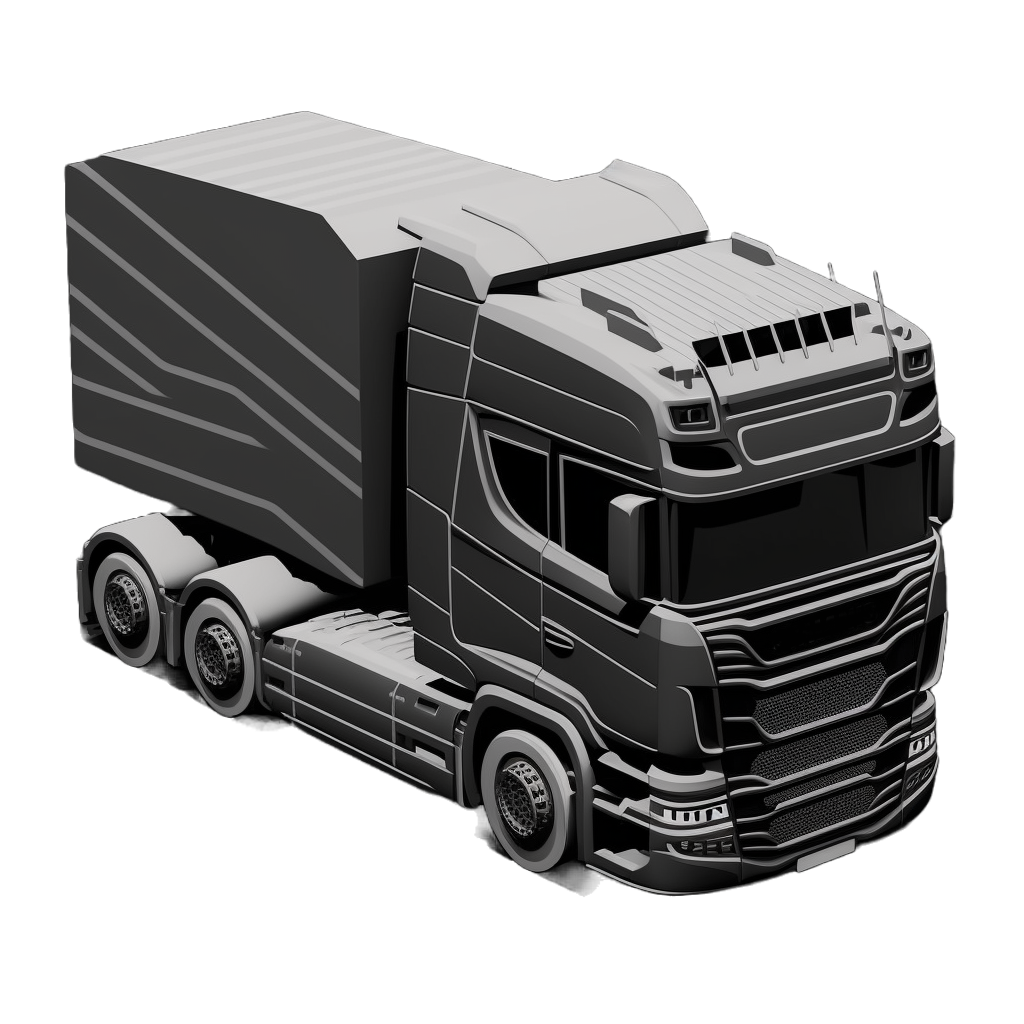
\includegraphics[width=.2\textwidth]{Images/scania-truck.png}};

\node[inner sep=0pt,left = \spacex of truck2] (truck1) {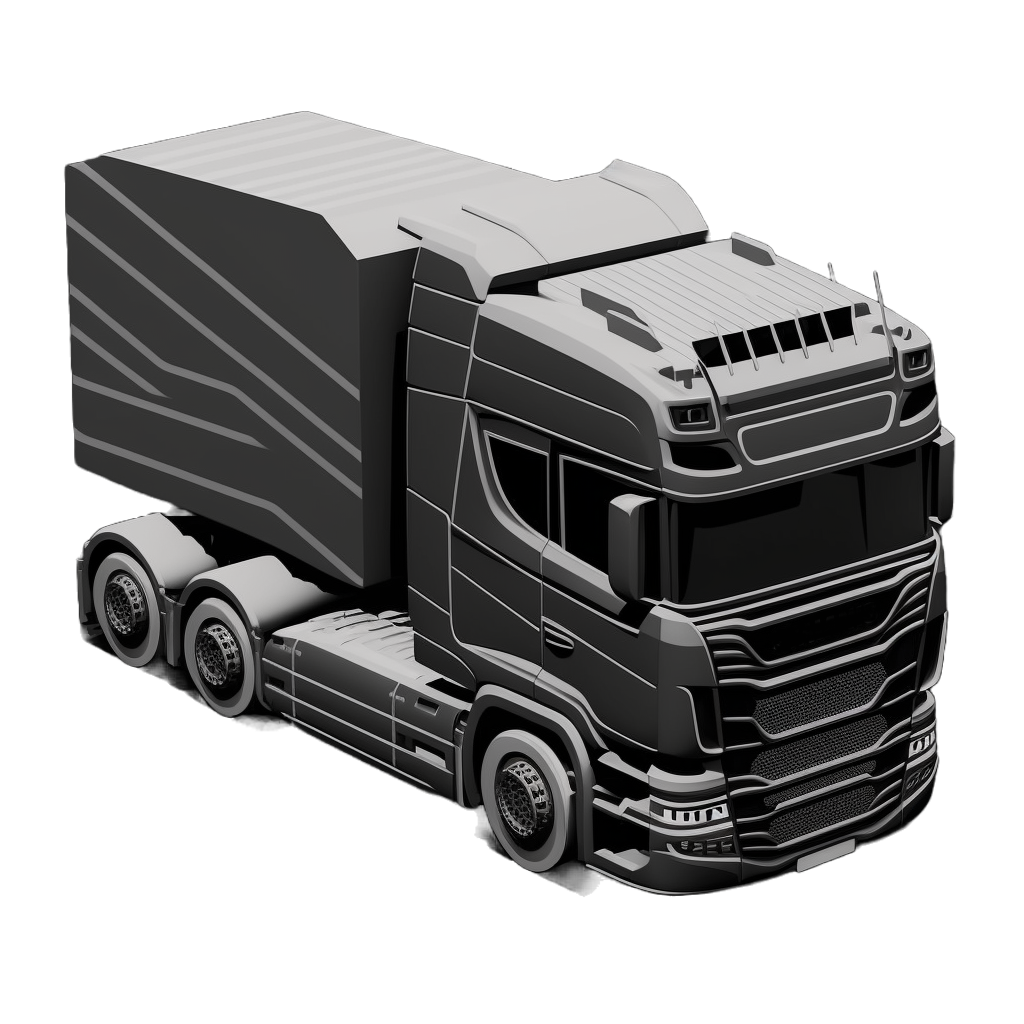
\includegraphics[width=.2\textwidth]{Images/scania-truck.png}};
\node[inner sep=0pt, right = \spacex of truck2] (truck3) {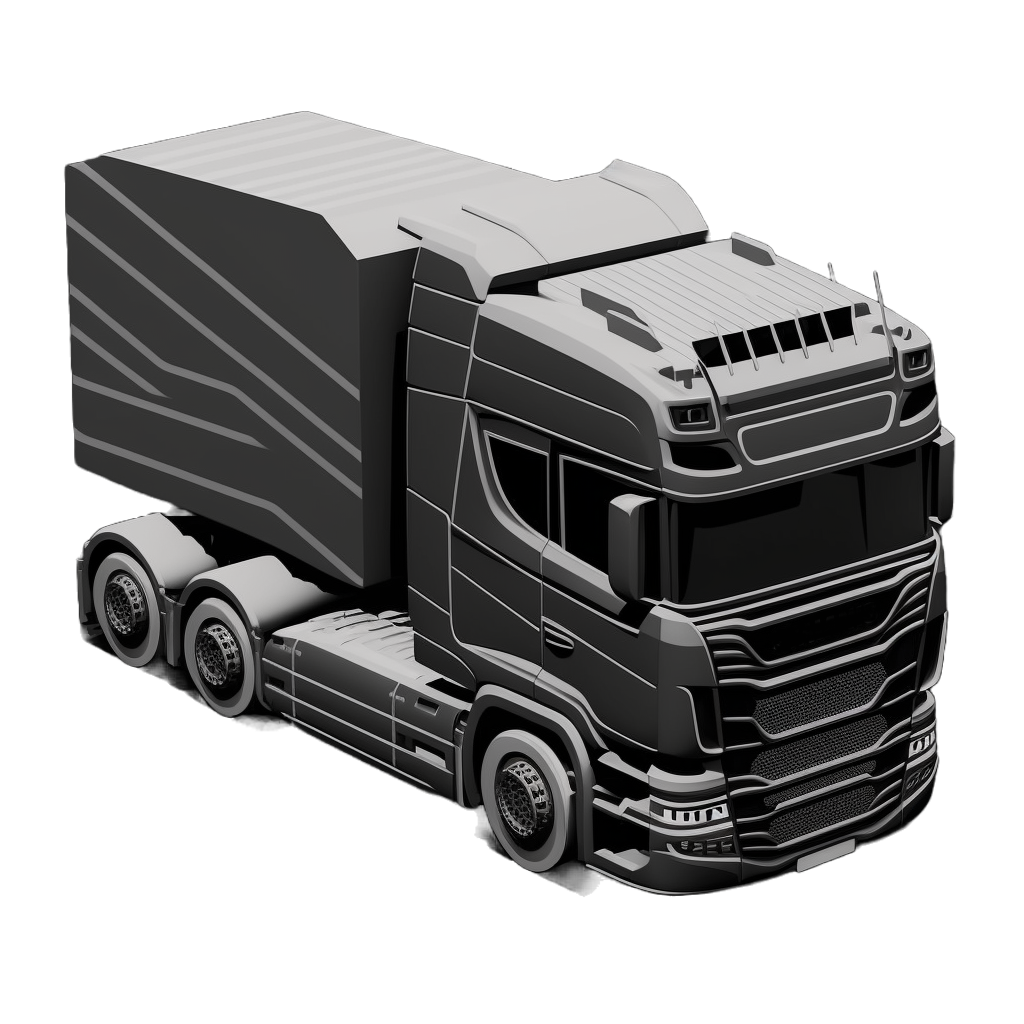
\includegraphics[width=.2\textwidth]{Images/scania-truck.png}};

\node[draw, above left = 0 and 0 of truck1,align=left,anchor = north west,fill=white,fill opacity = 0.7,fill=workcol] (work1) {\textbf{Feature \#1:} 19 - 36 \\ \textbf{Feature \#2:} 45  - 66};

\node[draw, above left = 0 and 0 of truck2,align=left,anchor = north west,fill=white,fill opacity = 0.7,fill=workcol] (work2) {\textbf{Feature \#1:} 23 - 29\\\textbf{Feature \#2:}  31 - 36};


\node[draw, above left = 0 and 0 of truck3,align=left,anchor = north west,fill=white,fill opacity = 0.7,fill=workcol] (work3) {\textbf{Feature \#1:} 26 - 41 \\ \textbf{Feature \#2:} 40 - 55};

\draw[arrow,myred] (serv.180) to [bend right] node[above,sloped,align=center] {19 - 41 \\ 31  - 66} (work1.100);
\draw[arrow] (work1.80) to node[below,sloped,align=center] {19 - 36 \\ 45  - 66} (serv.185);

\draw[arrow,myred] (serv.0) to [bend left] node[above,sloped,align=center] {19 - 41 \\ 31  - 66} (work3.80);
\draw[arrow] (work3.100) to node[below,sloped,align=center] {26 - 41 \\ 40  - 55} (serv.-5);

\draw[arrow] (work2.80) to node[above,sloped,align=center] {23 - 29 \\ 31  - 36} (serv.280);
\draw[arrow,myred] (serv.260) to [bend right] node[above,rotate=180,sloped,align=center] {19 -41 \\ 31 - 66} (work2.100);

\end{tikzpicture}
    \caption{Decentralized data normalization based on workers' minimum and maximum feature values.}
    \label{fig:normalize}
\end{figure}

\subsection{Decentralized Training Sequence}
%
\textcolor{blue}{In the decentralized training sequence of our time-series \gls*{gan} model, we employ the Adam optimizer with a learning rate of 2e-4, and parameters $\beta1$ = 0.5, $\beta2$ = 0.999 for both generator and discriminator. We found that \gls*{mse} loss outperformed \gls*{bce}, especially in a decentralized setting. The noise dimension for the generator was set to 128 and the batch size used was 4. Our testing showed that in our decentralized training setup, overriding the models with the winning discriminator led to a degradation in performance. Therefore, the chosen worker does not override the other workers.} The full training sequence of the decentralized time-series \gls*{gan} model involves the following steps:
%
\begin{itemize}
\item For each epoch, a target sequence width is determined in order to calculate the necessary noise size and actual sequence width output from the generator.
\item Random noise is generated and used to create fake sequences, which are then sent to all workers.
\item Workers create samples from their local real data that match the sequence width of the fake data received.
\item During each iteration, workers feed their discriminator a real sample with a target of one, and then feed it a fake sample with a target of zero.
\item Loss is calculated for both the real and fake data using \gls*{mse} loss. The overall loss for each discriminator is the average of both losses.
\item The overall loss is back-propagated to improve each discriminator using Adam optimizer~\cite{adam_optimizer}.
\item The fake losses for all workers are compared, and based on the training strategy either:
\begin{itemize}
\item The worker with the highest/lowest loss is chosen.
\item The weighed average of all discriminator parameters is used to create a global discriminator. % that overrides all the discriminators at each iteration.
\end{itemize}
\item The chosen worker's discriminator or the global discriminator's output on the fake data is used to calculate the loss of the generator with a target of one.
\item The generator loss is used to back-propagate and improve the generator using Adam optimizer.
\item Steps repeat with a different target sequence width.
\end{itemize}


\subsection{Evaluation Metrics}

\textcolor{blue}{In the early stages of our project, while the model was primarily designed for image data, we used established evaluation metrics such as the \gls*{fid} score. The \gls{fid} score is a popular choice for evaluating the quality of images generated by \glspl*{gan}. However, as we shifted our focus to time-series data, it became clear that the \gls{fid} score is not directly applicable in this new context. This necessitated the development of a new evaluation methodology tailored to time-series data.}

\textcolor{blue}{Consequently, we decided to implement an auto-regressive model as a primary evaluation measure. Auto-regression is a tried and tested method for the analysis and forecasting of time-series data and has proven effective as a performance metric for time-series forecasting models~\cite{rnntimeseries}. This auto-regressive approach allows for the evaluation of a \gls*{gan} model in three distinctive ways: \cite{esteban2017realvalued}}

\textcolor{red}{To quantitatively evaluate the time-series output, we used an autoregressive model. Autoregression is often used to analyze and forecast time-series data, and can be used as a metric for evaluating the performance of a forecasting model~\cite{rnntimeseries}. For \gls*{gan}, this can be done in 3 different ways:} %. Figure \ref{fig:trtr} visualizes those methods and they are as follows:
\begin{itemize}
    \item \textit{\gls*{trtr}:} Using only real data is useful to establish a baseline that determines how well the model is able to capture the statistical properties of the real data. This can then be used to validate the performance of the other methods.
    \item \textit{\gls*{trts}:} Instead of testing on real data, the synthetic data generated by the 
    \gls*{gan} model is used. This checks if the \gls*{gan} model has learned the underlying structure of the real data effectively.
    \item \textit{\gls*{tstr}:} This is opposite of the previous method and will be used as a secondary metric. The method determines if the synthetic data generated by the \gls*{gan} is of sufficient quality to be used in place of real data for training purposes.
\end{itemize}

%In our qualitative evaluation, we visually inspected the sequence output and further employed the use of \gls*{pca} by calculating it for both the real and synthetic data to visualize if the \gls*{gan} model has accurately captured the real data distribution.


%\def\trtrscale{0.6}
%\begin{table}[t]
\centering
\caption{TRTR results for each data behaviour}
\label{tab:trtr-main}
% \resizebox{\columnwidth}{!}{%

\begin{tabular}{lccc}
\Xhline{1.5pt}
\multicolumn{1}{c}{\multirow{2}{*}{\sc{Data Type}}} & \multicolumn{3}{c}{\sc{TRTR}} \\
\multicolumn{1}{c}{} & \sc{R2} & \sc{MAE} & \sc{RMSE} \\ \Xhline{1.2pt}
Anomalous  & 0.588       & 0.062        & 0.165         \\ \hline
Normal     & 0.819       & 0.039        & 0.104         \\ \hline
Mixed      & 0.530       & 0.071        & 0.172         \\\Xhline{1.5pt}
\end{tabular}%
% }
\end{table}

\section{Results}
% All this Sec.~will be 1/2 pages.


%The testing process began with a single worker (centralized \gls*{gan}) in order to determine the optimal layer architecture for the generator and discriminator. We initially conducted the testing using anomalous data, and then normal data was introduced later on.
We compared the performance of centralized \gls*{gan} (i.e., a single worker) with our decentralized approach. 
For evaluation, we trained 3 separate auto-regression models \gls*{trtr} for each data behaviour (normal, anomalous, mixed). Each \gls*{trtr} model is needed to calculate the corresponding \gls*{trts} for the \gls*{gan} getting tested. The auto-regression models are set-up to predict the last five time steps.
%
As shown in Tab.~\ref{tab:trtr-main}, the regression model has a higher R2 score when applied to the normal behaviour data-set. This suggests that the model is more accurate on normal data rather than anomalous or mixed ones. We use the \gls*{trtr} metric to verify the results when applied to synthetic data. In particular, we tested each \gls*{trtr} on 10 different synthetic data samples from each generator to calculate an average for the \gls*{trts} metric. Similarly, we trained an auto-regression model with synthetic data 10 different times to calculate an average for the \gls*{tstr} metric.

\begin{table}[t]
\centering
\caption{TRTR results for each data behaviour}
\label{tab:trtr-main}
% \resizebox{\columnwidth}{!}{%

\begin{tabular}{lccc}
\Xhline{1.5pt}
\multicolumn{1}{c}{\multirow{2}{*}{\sc{Data Type}}} & \multicolumn{3}{c}{\sc{TRTR}} \\
\multicolumn{1}{c}{} & \sc{R2} & \sc{MAE} & \sc{RMSE} \\ \Xhline{1.2pt}
Anomalous  & 0.588       & 0.062        & 0.165         \\ \hline
Normal     & 0.819       & 0.039        & 0.104         \\ \hline
Mixed      & 0.530       & 0.071        & 0.172         \\\Xhline{1.5pt}
\end{tabular}%
% }
\end{table}


\subsection{Centralized GAN Results}

We tested the \gls*{gan} model initially using fixed sequence widths of 64, 128, and 256 seconds. The results show a sequence width of 64 seconds being the better performer if we used the fixed sequence strategy width. After applying the dynamic window strategy, both visual inspection and the \gls*{trts} / \gls*{tstr} (see Tab.~\ref{tab:dynamic-window}) showed an improvement. This confirms that the dynamic window in fact improves the capabilities of the generator in contrast to using a fixed sequence width.

\begin{table}[t]
\centering
\caption{Dynamic window effect (anomalous behaviour)}\marginnote{\textcolor{blue}{RC22}}
\label{tab:dynamic-window}
%\resizebox{\columnwidth}{!}{%
\begin{tabular}{lcccccc}
\Xhline{1.5pt}
\multicolumn{1}{c}{\multirow{2}{*}{\sc{\begin{tabular}[c]{@{}c@{}}Sequence \\ Width\end{tabular}}}} &
  \multicolumn{3}{c}{\sc{TRTS}} &
  \multicolumn{3}{c}{\sc{TSTR}} \\
\multicolumn{1}{c}{} &
  \sc{R2} &
  \sc{MAE} &
  \sc{RMSE} &
  \sc{R2} & 
  \sc{MAE} &
  \sc{RMSE} \\ \Xhline{1pt}
64 s  & 0.375 & 0.089 & 0.203 & 0.609 & 0.055	& 0.160 \\ \hline
128 s & 0.352 & 0.084 & 0.206 & 0.599 & 0.054	& 0.165 \\ \hline
256 s & 0.153 & 0.177 & 0.236 & -1.84 & 0.215	& 0.284 \\\hline
Dynamic     & 0.550 & 0.070 & 0.171 & 0.621 & 0.051 & 0.162\\ \Xhline{1.6pt}
\textcolor{blue}{TimeGAN}     & \textcolor{blue}{0.471}	& \textcolor{blue}{0.073}	& \textcolor{blue}{0.187}	& \textcolor{blue}{0.604}	& \textcolor{blue}{0.057}	& \textcolor{blue}{0.162}\\ \Xhline{1.5pt}
\end{tabular}%
%}
\end{table}





%
The normalization we used in previous tests employed the first technique mentioned in Sec.~\ref{sec:data-pre-process}, where each feature is normalized based on the known capabilities of that specific feature. We then further tested the second technique, where the normalization occurs based on the limits of the workers. The \gls*{trts} / \gls*{tstr} results in Tab.~\ref{tab:normalize-result} showed that using the worker limits yields a significant improvement. We adapted the second technique to all upcoming tests.
\begin{table}[t]
\centering
\caption{Worker normalization effect (normal behaviour)}
\resizebox{\columnwidth}{!}{%
\begin{tabular}{lcccccc}
\Xhline{1.5pt}
\multicolumn{1}{c}{\multirow{2}{*}{\sc{Normalization}}} & \multicolumn{3}{c}{\sc{TRTS}} & \multicolumn{3}{c}{\sc{TSTR}} \\ 
\multicolumn{1}{c}{}    & \sc{R2}    & \sc{MAE}   & \sc{RMSE}  & \sc{R2}    & \sc{MAE}   & \sc{RMSE}  \\ \Xhline{1.2pt}
Fixed Limits  &  0.472	& 0.096	& 0.169	& 0.743	& 0.133	& 0.164 \\ \hline
Worker Limits &  0.724	& 0.041	& 0.128	& 0.901	& 0.028	& 0.070 \\ \Xhline{1.5pt}
\end{tabular}%
}

\label{tab:normalize-result}
\end{table}






\subsection{Decentralized GAN Results}
%
We set-up the network with one server and four workers. Workers \#1 and \#2 had anomalous data, while workers \#3 and \#4 had normal data.
As shown in Fig.~\ref{fig:decentralized_results}, the output sequence generated by the most forgiving strategy only contain behaviour belonging to workers \#1 and \#2 (Anomalous), while the least forgiving strategy produces a mix of classes from both workers. This output shows both normal and anomalous behaviour, which looks similar to the mixed data behaviour shown in Fig.~\ref{fig:scania-data}. This can also be corroborated by examining the worker contribution count, which tracks the number of times each worker was selected for generator training (see Fig.~\ref{fig:work-cont-decentralized}. The most forgiving strategy exhibits a strong bias towards workers \#1 and \#2, while the least forgiving strategy exhibits a more balanced distribution. This explains the difference in output observed in the generated sequences.

\begin{table}[t]

\centering
\caption{FL strategy effect (mixed behaviour)}
\resizebox{\columnwidth}{!}{%
\begin{tabular}{lcccccc}
\Xhline{1.5pt}
\multicolumn{1}{c}{\multirow{2}{*}{\sc{FL Strategy}}} & \multicolumn{3}{c}{\sc{TRTS}} & \multicolumn{3}{c}{\sc{TSTR}} \\ 
\multicolumn{1}{c}{}    & \sc{R2}    & \sc{MAE}   & \sc{RMSE}  & \sc{R2}    & \sc{MAE}   & \sc{RMSE}  \\ \Xhline{1.2pt}

Most Forgiving & 0.504 & 0.070 & 0.176 & 0.426 & 0.067 & 0.177 \\  \hline
Weighted Average & 0.348 & 0.090 & 0.201 & 0.522 & 0.071 & 0.170 \\ \hline
Least Forgiving & 0.525	& 0.076	& 0.172	& 0.588	& 0.055	& 0.158 \\
\Xhline{1.5pt}

\end{tabular}
}

\label{tab:decentralized-tstr}
\end{table}





The behaviour of the most forgiving strategy can be understood as follows; in this approach, the generator is updated based on the worker with the highest loss on the fake data produced by the generator. This leads to the generator creating fake data that closely resembles the data of the selected worker. In subsequent iterations, it is expected that the previously selected worker will have a higher loss on the fake images, as the generator is more specialized to their data. On the other hand, the rest of the workers are likely to have a lower loss, insuring a much less likelihood of being selected. As the training process continues, the generator is expected to converge on a small subset of workers, effectively ignoring the data of other workers as the distribution of generated data is very different from their local data distribution. 

We also implemented and tested two different forms of weighting for the averaging technique (\gls*{f2a}), one that favoured the most forgiving worker and another that favoured the least forgiving worker. We used the Softmax function to determine the contribution of each worker to the overall average model. In the next iteration, all workers used the newly averaged discriminator model. However, there was a noticeable output degradation as suggested by the \gls*{trts} / \gls*{tstr} results and the output sequence shown in Fig.~\ref{fig:decentralized_results}.
%
\def\layerfigwidth{0.8}
\def\layerfigheight{0.25}
\def\ydist{-3.7}
\begin{figure} [t]
    \centering
\begin{tikzpicture}[scale = 0.61]
\begin{axis} [every axis plot post/.append style={mark=none,smooth,-,line width = \plotlinewidth pt},
ylabel={Most Forgiving},
axis x line=bottom,
axis y line=left,
axis line style={-,line width = 1pt},
% ticks=none,
width=\layerfigwidth\textwidth,
height=\layerfigheight\textwidth,
xmax = 1000,
ymax=1.005
] 
    \addplot[fone] table [col sep=comma,header=true,x index=0,y index=1] {Data/most_forgiving.csv};
    \addplot[ftwo] table [col sep=comma,header=true,x index=0,y index=2] {Data/most_forgiving.csv};
    \addplot[fthree] table [col sep=comma,header=true,x index=0,y index=3] {Data/most_forgiving.csv};
    \addplot[ffour] table [col sep=comma,header=true,x index=0,y index=4] {Data/most_forgiving.csv};
    \addplot[ffive] table [col sep=comma,header=true,x index=0,y index=5] {Data/most_forgiving.csv};  
    \addplot[fsix] table [col sep=comma,header=true,x index=0,y index=6] {Data/most_forgiving.csv};
    \addplot[fseven] table [col sep=comma,header=true,x index=0,y index=7] {Data/most_forgiving.csv};
    \addplot[feight] table [col sep=comma,header=true,x index=0,y index=8] {Data/most_forgiving.csv};
\end{axis}


\begin{axis} [at={(0,\ydist cm)},every axis plot post/.append style={mark=none,smooth,-,line width = \plotlinewidth pt},
% xlabel={Time Step [s]},
ylabel={Weighted Average},
axis x line=bottom,
axis y line=left,
axis line style={-,line width = 1pt},
% ticks=none,
width=\layerfigwidth\textwidth,
height=\layerfigheight\textwidth,
xmax = 1000,
ymax=1.005
]
    \addplot[fone] table [col sep=comma,header=true,x index=0,y index=1] {Data/weighted_avg.csv};
    \addplot[ftwo] table [col sep=comma,header=true,x index=0,y index=2] {Data/weighted_avg.csv};
    \addplot[fthree] table [col sep=comma,header=true,x index=0,y index=3] {Data/weighted_avg.csv};
    \addplot[ffour] table [col sep=comma,header=true,x index=0,y index=4] {Data/weighted_avg.csv};
    \addplot[ffive] table [col sep=comma,header=true,x index=0,y index=5] {Data/weighted_avg.csv};  
    \addplot[fsix] table [col sep=comma,header=true,x index=0,y index=6] {Data/weighted_avg.csv};
    \addplot[fseven] table [col sep=comma,header=true,x index=0,y index=7] {Data/weighted_avg.csv};
    \addplot[feight] table [col sep=comma,header=true,x index=0,y index=8] {Data/weighted_avg.csv};
\end{axis}

\begin{axis} [at={(0,\ydist*2 cm)},every axis plot post/.append style={mark=none,smooth,-,line width = \plotlinewidth pt},
xlabel={Time Step [s]},
ylabel={Least Forgiving},
axis x line=bottom,
axis y line=left,
axis line style={-,line width = 1pt},
% ticks=none,
width=\layerfigwidth\textwidth,
height=\layerfigheight\textwidth,
xmax = 1000,
ymax=1.005,
legend columns=4,
legend style={at={(0.5,-0.5)},anchor=north,font=\large}
]
    \addplot[fone] table [col sep=comma,header=true,x index=0,y index=1] {Data/least_forgiving_2.csv};
    \addplot[ftwo] table [col sep=comma,header=true,x index=0,y index=2] {Data/least_forgiving_2.csv};
    \addplot[fthree] table [col sep=comma,header=true,x index=0,y index=3] {Data/least_forgiving_2.csv};
    \addplot[ffour] table [col sep=comma,header=true,x index=0,y index=4] {Data/least_forgiving_2.csv};
    \addplot[ffive] table [col sep=comma,header=true,x index=0,y index=5] {Data/least_forgiving_2.csv};  
    \addplot[fsix] table [col sep=comma,header=true,x index=0,y index=6] {Data/least_forgiving_2.csv};
    \addplot[fseven] table [col sep=comma,header=true,x index=0,y index=7] {Data/least_forgiving_2.csv};
    \addplot[feight] table [col sep=comma,header=true,x index=0,y index=8] {Data/least_forgiving_2.csv};
    \legend{Feature \#1,Feature \#2,Feature \#3,Feature \#4,Feature \#5,Feature \#6,Feature \#7,Feature \#8}
\end{axis}

\end{tikzpicture}
\caption{The output of our decentralized GAN for non-IID APS data.}
\label{fig:decentralized_results}
\end{figure}



%
\def\jumper{3}
\def\increase{1.5}
\begin{figure}[t]
    \centering
\begin{tikzpicture}[line width = 1pt,line cap=round, line join=round,anchor=center, font=\footnotesize]  
\begin{axis}[
    ybar, 
    % bar width=20pt,
    ylabel={Contribution},
    xlabel={Training Strategy},
    axis x line*=bottom,
    axis y line=left,
    xtick={1,1+\jumper,1+\jumper*2},
    xticklabel style   = {align=center},
    xticklabels={Most Forgiving, Weighted Avg, Least Forgiving},
    axis line style={-,line width = 1pt},
    width=0.5\textwidth,
    height=0.28\textwidth,
    xmin =  1-\increase,
    xmax = \increase+1+\jumper*2,
    scaled ticks=false,
    ymin= 0,
    ymax = 100000,
    ytick=\empty,
    legend cell align={left},
    % legend style={at={(0.6,1)},anchor=north},
    ]


\addplot [fill=myblue ,line width = 1pt] coordinates{
   (1,71000)
   (1+\jumper,35000)
   (1+\jumper*2,32000)};
\addplot [fill=orange ,line width = 1pt] coordinates{
   (1,67000)  
   (1+\jumper,35000)
   (1+\jumper*2,41000)};

\addplot [fill=Emerald ,line width = 1pt] coordinates{
   (1,2300)
   (1+\jumper,35000)
   (1+\jumper*2,33000)};
\addplot [fill=myred ,line width = 1pt] coordinates{
   (1,800)
   (1+\jumper,35000)
   (1+\jumper*2,34000)};

   
\legend{Worker \#1 [Anomalous],Worker \#2 [Anomalous],Worker \#3 [Normal],Worker \#4 [Normal] }
   
\end{axis}    
\end{tikzpicture}
    \caption{Worker contribution based on training strategy.}
    \label{fig:work-cont-decentralized}
\end{figure}
%
%\def\scale{1}

\begin{figure}[t]
    \centering
    \subfloat[Most Forgiving]{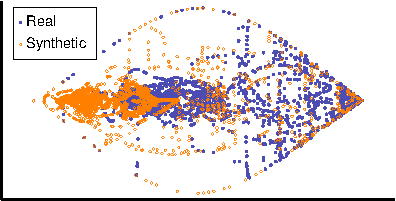
\includegraphics[scale=\scale]{Images/pca-mf.pdf}}
    \hfill
    \subfloat[Least Forgiving]{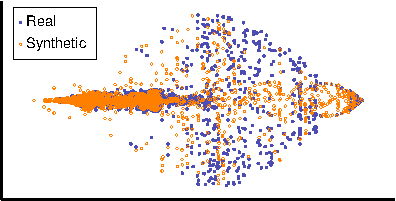
\includegraphics[scale=\scale]{Images/pca-lf.pdf}}
    \caption{PCA output of real vs. synthetic mixed data based on FL strategy.}
    \label{fig:pca-decentralized}
\end{figure}




\section{Conclusion and Future Work}
% 1/1.5 columns.

%We first visually evaluated the performance of the time-series based \gls*{gan} by examining the output and comparing the \gls*{pca} of the real and synthetic data. We performed the quantitative evaluation using auto-regression models trained on three types of behaviour data (anomalous, normal, mixed). We then calculated the \gls*{trts} and \gls*{tstr} metrics using these models.

We presented an approach to generate synthetic anomalous vehicle sensor data that combines \gls*{gan} and \gls*{fl} to preserve the privacy of personal information. For the training strategies, %we compared the most and least forgiving. The most forgiving produced an output that only contained classes belonging to one behaviour, while the least forgiving produced a mix of classes from the available behaviours. This concluded that the most forgiving strategy consistently over-fits to a particular worker. This result was unexpected, as it did not align with the performance of the previously proposed \gls*{f2u} architecture in \cite{yonetani_decentralized_2019}. When the parameters of the winning discriminator were allowed to override the other workers' parameters, the behaviour of the two strategies was reversed. However, the output quality was significantly degraded in this case.
%
we evaluated the two forms of the weighted averaging (\gls*{f2a}) technique, namely most and least forgiving. %, and both performed similarly. There was however a significant degradation in the output compared to the most and least forgiving strategies.
%
We found the least forgiving training strategy to be the most effective in decentralized learning. It was able to maintain stable and non-divergent training, even with \gls*{niid} data. Additionally, the generated data produced by this strategy included all classes represented by the different workers, indicating good generalization capability. Furthermore, the generated features maintained the same correlations exhibited in the real data.
%
Testing concluded that the dynamic window strategy and normalization based on worker limits both improved the performance of the output. 

%\atB{I would shorten the following in a paragraph of $\leq 10$ lines.}

In our future research, we plan to employ the use of \textit{model compression} to reduce the size of the model while maintaining its performance level~\cite{hinton2015distilling} and to investigate the applicability of \textit{diffusion models}~\cite{alcaraz_diffusion-based_2022} to federated learning scenarios.

% There are multiple opportunities for enhancement and areas for further exploration. The following list outlines several avenues for future research:


% \begin{itemize}
%     \item \textbf{Model compression:} Refers to the process of reducing the size of an \gls*{ml} model, while maintaining its performance and making it more compatible with edge devices. There are several methods of model compression, including pruning and knowledge distillation \cite{ye_three_2021}.
%     \item \textbf{Diffusion models:} Investigate the use of diffusion models in an \gls*{fl} architecture to generate time-series data. They have been wildly successfully in image generation and time-series forecasting \cite{alcaraz_diffusion-based_2022}. In \cite{rasul2021autoregressive}, the authors presented a novel approach that combines auto-regressive modeling and de-noising diffusion models to effectively capture the dependencies and noise structure in multivariate time series data. Their proposed method demonstrates improved performance compared to existing state-of-the-art techniques in time series forecasting when tested on various benchmarks and real-world data-sets. 

% \end{itemize}

% \atB{Please check which papers have been published in a proper venue (e.g., conferences, journals, etc.). Arxiv is a collection of non-peer-reviewed paper and we should acknowledge effort to publish in real venues}


\bibliographystyle{IEEEtran}
%\bibliography{Master_Thesis}
\textcolor{red}{\marginnote{RC13}
\bibliography{simplebib}}

\end{document}


